%% Copernicus Publications Manuscript Preparation Template for LaTeX Submissions
%% ---------------------------------
%% This template should be used for copernicus.cls
%% The class file and some style files are bundled in the Copernicus Latex Package, which can be downloaded from the different journal webpages.
%% For further assistance please contact Copernicus Publications at: production@copernicus.org
%% https://publications.copernicus.org/for_authors/manuscript_preparation.html


%% Please use the following documentclass and journal abbreviations for preprints and final revised papers.

%% 2-column papers and preprints
\documentclass[journal abbreviation, manuscript]{copernicus}



%% Journal abbreviations (please use the same for preprints and final revised papers)


% Advances in Geosciences (adgeo)
% Advances in Radio Science (ars)
% Advances in Science and Research (asr)
% Advances in Statistical Climatology, Meteorology and Oceanography (ascmo)
% Annales Geophysicae (angeo)
% Archives Animal Breeding (aab)
% ASTRA Proceedings (ap)
% Atmospheric Chemistry and Physics (acp)
% Atmospheric Measurement Techniques (amt)
% Biogeosciences (bg)
% Climate of the Past (cp)
% DEUQUA Special Publications (deuquasp)
% Drinking Water Engineering and Science (dwes)
% Earth Surface Dynamics (esurf)
% Earth System Dynamics (esd)
% Earth System Science Data (essd)
% E&G Quaternary Science Journal (egqsj)
% European Journal of Mineralogy (ejm)
% Fossil Record (fr)
% Geochronology (gchron)
% Geographica Helvetica (gh)
% Geoscience Communication (gc)
% Geoscientific Instrumentation, Methods and Data Systems (gi)
% Geoscientific Model Development (gmd)
% History of Geo- and Space Sciences (hgss)
% Hydrology and Earth System Sciences (hess)
% Journal of Bone and Joint Infection (jbji)
% Journal of Micropalaeontology (jm)
% Journal of Sensors and Sensor Systems (jsss)
% Magnetic Resonance (mr)
% Mechanical Sciences (ms)
% Natural Hazards and Earth System Sciences (nhess)
% Nonlinear Processes in Geophysics (npg)
% Ocean Science (os)
% Polarforschung - Journal of the German Society for Polar Research (polf)
% Primate Biology (pb)
% Proceedings of the International Association of Hydrological Sciences (piahs)
% Scientific Drilling (sd)
% SOIL (soil)
% Solid Earth (se)
% The Cryosphere (tc)
% Weather and Climate Dynamics (wcd)
% Web Ecology (we)
% Wind Energy Science (wes)


%% \usepackage commands included in the copernicus.cls:
%\usepackage[german, english]{babel}
%\usepackage{tabularx}
%\usepackage{cancel}
%\usepackage{multirow}
%\usepackage{supertabular}
%\usepackage{algorithmic}
%\usepackage{algorithm}
%\usepackage{amsthm}
%\usepackage{float}
%\usepackage{subfig}
%\usepackage{rotating}


\usepackage{comment} 
\usepackage{enumerate}

\begin{document}

\title{Phydra 0.1: an open source Python library using the XSO framework for flexible, modular and reproducible marine ecosystem modeling based on ordinary differential equations} 


% \Author[affil]{given_name}{surname}
\Author[1]{Benjamin}{Post}
\Author[1]{Esteban}{Acevedo-Trejos}
\Author[2]{Andrew }{Barton}
\Author[3]{Benoît}{Bovy}
\Author[1]{Agostino}{Merico}



\affil[1]{Leibniz Centre for Tropical Marine Research (ZMT), Bremen, Germany}
\affil[2]{Scripps Institution of Oceanography, La Jolla, CA, United States}
\affil[3]{GFZ German Research Centre for Geosciences, Potsdam, Germany}


%% The [] brackets identify the author with the corresponding affiliation. 1, 2, 3, etc. should be inserted.

%% If an author is deceased, please mark the respective author name(s) with a dagger, e.g. "\Author[2,$\dag$]{Anton}{Aman}", and add a further "\affil[$\dag$]{deceased, 1 July 2019}".

%% If authors contributed equally, please mark the respective author names with an asterisk, e.g. "\Author[2,*]{Anton}{Aman}" and "\Author[3,*]{Bradley}{Bman}" and add a further affiliation: "\affil[*]{These authors contributed equally to this work.}".


\correspondence{Benjamin Post (benjamin.post@leibniz-zmt.de)}


\runningtitle{phydra v1}

\runningauthor{Post}





\received{}
\pubdiscuss{} %% only important for two-stage journals
\revised{}
\accepted{}
\published{}

%% These dates will be inserted by Copernicus Publications during the typesetting process.

\firstpage{1}

\maketitle

\begin{abstract} [Just collecting ideas:] 

Marine ecosystem modeling is central to understanding the biogeochemical cycles driving the earth system. 

These models can have highly variable complexity, both in terms of mechanistic and spatial resolution. 
No consensus in terms of adequate model complexity and formulation has been reached, although there are many canonical model structures used and modified.

This paper introduces Phydra, an open-source library for marine ecosystem modeling built with the object-oriented modeling framework Xarray-simlab-ODE (XSO), with the goal to support efficient, flexible and easily reproducible development of models based on ordinary differential equations. 

Phydra provides pre-built models and model components that can be modified and assembled to complex ecosystem models. 

All basic processes can be adapted and modified in simple Python to describe different and more complex ecosystems. The first release focuses on zero-dimensional phytoplankton models, but models of higher dimensionality are also possible.

Xarray data-structure, self-documenting workflow, ease of sharing models, as well as input and output.

Phydra is embedded in the Python scientific ecosystem and is natively compatible with many tools for prototyping, analysis \& visualisation of models.

This paper presents the general structure of Phydra, the usage of xarray-simlab-ode and the workflow of developing model applications of varying complexity.

Phydra, as well as all models and other work presented here is available open-source and can be used by the scientific community to build, modify, run and test ODE-based models. The Phydra standard library aspect, can collaborate share model functions mechanisms, really focus on science instead of fixing bugs.. 

Comprehensive documentation is available online.





% Through the combination of the XSO framework and the Phydra library, a high level of customisation and flexibility is combined with less boilerplate code and technical setup.

%Phydra is a Python package, embedded in the Python scientific ecosystem and is natively compatible with many tools for prototyping, analysis \& visualisation of models.

%, allowing modelers to simplify the model construction and focus on the scientific questions.

%Xarray-simlab-ODE provides a framework based on compact python classes and custom variables to define systems of ordinary or partial differential equations, that can be used with different solvers.


%Here, we demonstrate the usage of the phydra v1 package in a simple NPZD setting and to showcase the flexibility, in a more complex size based trophic structure model. Both in slab physics.

%The utility of the phydra package is here shown via three model implementations. Two models from literature are recreated, and the flexible nature of this package allows a combination of as a third example. 
\end{abstract}


\copyrightstatement{TEXT} %% This section is optional and can be used for copyright transfers.

%%% added Section for editing purposes, later simply use \introduction
\section{Introduction}
%\introduction  %% \introduction[modified heading if necessary]

% introduction should be adundantly clear with no unecessary details!
% can also mention open source, but just high-level summaries, same on phydra details, no detail in intro
% establish, why what you make is different from everything done before. why it is important! (2 sentences)

% 2nd Section:
% Background, theoretical framework. Specifics here!

% FIRST SECTION: general info - Biogeochemical role of phytoplankton

%- P1: why phytoplankton important?
\subsection{Models of marine ecosystems}
- major primary producers ocean ecosystem, understanding important, global change (important part of climate models)

These microorganisms form the basis of the food webs, and contribute roughly half of the oxygen in our atmosphere through photo- synthesis \citep{Field2009}.

The biomass produced indirectly feeds a considerable part of earth’s population through fisheries \citep{Stock2017} and also shapes the elemental composition of oceanic water itself \citep{Redfield1958}.

A small fraction of primary production sinks out of the photic layer as fecal pellets or detrital matter, to the deeper ocean, and an even smaller fraction reaches the sea floor as sediment (\~ 1 \%) and is finally removed from the system over geological times \citep{Honjo2008}. Carbon sequestered this way is removed from the ocean-atmosphere system for potentially millions of years.

- phytoplankton diversity 
Originating from several major phyla, there are estimated to be at least 25,000 species of phytoplankton \citep{Falkowski2004a} spanning over nine orders of magnitude in cell size \citep{Sieburth1978PelagicFractions, Finkel2010}.

- complex system --> complex models?! dealing with highly dimensional models \citep{Dutkiewicz2020DimensionsDiversity}


%  \subsection{Phytoplankton modeling: From NPZD to DARWIN}
%- P2: why people model phytoplankton? (what are the types of model we use? npzd, pft, size, darwin, etc.)
- based on ordinary diff equations!

- quote Gentleman history of marine ecosystem modeling \citep{Gentleman2003a}

- cite the beautiful paper on Steele's legacy \citep{Anderson2019RememberingEcosystems}

Given the complexity of the ocean ecosystem, it is necessary to aggregate our knowledge of the many smaller parts into comprehensive ecological models in order to understand the full-scale implications. Computational models of phytoplankton growth have been developed since the 1970s and have greatly increased in sophistication and complexity since then, co-evolving with the rise in computational resources. Ecosystem modelling started with simple box-model descriptions of a few trophic levels. These were the nutrient-phytoplankton-zooplankton (NPZ) and nutrient-phytoplankton-zooplankton-detritus (NPZD) models, which succeeded in reproducing the basic bloom dynamics observed in the temperate ocean \citep{Evans1985ACycles, Fasham1990a}. 

% \subsection{Running before we can walk}
% INSTEAD OF SUBSECTIONS; THESE ARE SIMPLY PARAGRAPHS

%- P3: all these different models, what is the problem? [Motivation for a better toolkit]
The simplicity of an NPZD model, where each of the four ecosystem components is represented by a single state variable, can be criticised as oversimplifying the complexity of a natural plankton community.

- These are very simplistic descriptions of ocean ecosystems, these models unavoidably limit the characterization of a diverse phytoplankton community [citation of Bruggeman?]. 

To make up for this shortcoming, in the following two decades, these models were expanded to more complex plankton functional type (PFT) models \citep{LeQuere2005}. For every group of species that fulfil a distinct ecosystem function, a new set of state variables and parameters was added, complicating the model structure and massively prolonging calculations. This somewhat intuitive approach of having every functional group represented in a model, however, did create problems. First and foremost, this is the lack and inherent uncertainty of data from field and culture experiments to constrain functional types. This again leads to the difficulty of validating the model output in light of insufficient information \citep{Shimoda2016}.

- Complex PFT models should not be initialized naively, but instead treated as hypotheses and multiple structures and levels of complexity should be tested against objective functions (usually data). \citep{Franks2009}

- Parameter identification in marine ecosystem models is complicated, but very important! \citep{Schartau2017}

- misleading legacies in phytoplankton modeling, formulations are routinely used that do not make physiological sense \citep{Smith2014}

and state: phydra is built with the idea in mind, that all ecosystem models are theories/hypotheses, that need to be tested against data, and tested against other models (particularly models of varying complexity). Occam's razor. 

- lots of models, in lots of (often old) programming languages, varying implementations
- all different, hidden (+very complex) codebase, not easy to adapt \& modify

ALTHOUGH, actually often very similar in nature and underlying technical processes, so if we could use a common framework that is sufficiently accessible and flexible, we can spend much less time on technicalities.

- but development in data science \& other computer science areas, towards reproducible tools, towards shared frameworks and capabilities (like Benoît said in his blog post: \href{https://medium.com/pangeo/pangeo-data-and-models-280b251ff0cd}{LINK} )

- tools should foster scientific collaboration
"easy to use, open source, easy to modify, toolbox"
- python Pangeo software ecosystem (jupyter, xarray, zarr)


\subsection{Open, flexible \& collaborative modeling}

%\subsection{Collaborative modelling using open source solution}
%- P4: Here's my solution! Here I present flexible model framework. explain basic structure and function

% can also mention open source, but just high-level summaries, same on phydra details, no detail in intro
% establish, why what you make is different from everything done before. why it is important! (2 sentences)

""In geosciences as well as in many other scientific domains, researchers rely more and more on the use of computer models to better understand complex phenomena. Yet, as new simulation experiments are designed and tested, the growing development of these models often leads to "monolithic" codes and i/o interfaces of increasing complexity, raising issues of maintainability and error-proneness.""

The tools used in academic computational modeling show a growing gap to the software ecosystems for data analysis. Perhaps in part due to the smaller user base, the former often have a steeper learning curve, are less accessible to novice users and can result in convoluted workflows. The latter is evolving rapidly towards more interactive and streamlined workflows.

Implementations of marine ecosystem models often evolve organically to higher complexities at the expense of their readability, which may compromise sustainability in the long term. In particularly, simplifying already complex models is not always possible or simple.

There are already some great modeling frameworks aimed to address the two issues above in the Python Scientific ecosystem (e.g., Climlab, CliMT/Simpl, Landlab), but there is to our knowledge no project to establish such a modeling framework in marine ecosystem modeling. \textit{[Not sure if this is true!]}

There have been different projects aimed at increasing the ease of model creation, both on the lower and higher-end. All projects have trade-offs, and what is most important is a common language and communication within the user community.
There are these.. and these projects (need some examples: Ecosym (?), Stella modeling tool (GUI), etc.).
Some of these proprietary software = not good!

Phydra is not designed to be specifically used with a graphical user interface (GUI), although such functionality could be added to the modular code base.
The design aims at allowing intuitive control of all levels of complexity, the base python code, mathematical solver implementations, as well as the higher level of assembling models from building blocks.

Why python? -> most popular programming language, rich scientific user community, Pangeo, rising language, relatively easy to learn

"Python is a high-level programming language well suited to rapid development and prototyping, as well as being more accessible to domain scientists than low-level languages such as FORTRAN or C++." - Mobius GMD paper
- This is also due to the dynamic interpretation of python, which makes python slower, but python is rapidly developing and leveraging other lower level language for speed. Also has growing functionality for parallelisation of code execution which is very relevant to large multi-dimensional marine ecosystem model use cases. 

Many large physical and ecological models are to this day written in FORTRAN. Due to the statically-typed nature it is more computationally efficient particularly for larger models. Yet despite it's speed, FORTRAN remains less accessible to scientists and usage and literacy of Python in the scientific community far exceeds that of FORTRAN.
Phydra is a project to bridge the gap between older, but more efficient ecosystem model code written in low-level languages like C++ and FORTRAN and the flexibility and usability of modern high-level programming languages. Python is a free and open-source language that is flexible, popular and has gained wide use in the scientific community. By being written in Python, Phydra can interact with a rich environment of popular scientific and numerical packages, and e.g. tools for machine learning. 


\subsection{Aims}
% AIM for phydra:
Why Phydra? -> collaborative development and open science are central to the Python project, no such previous tool available, but seems very much needed (see previous problems!)

Phydra is a library for those starting out with marine ecosystem modeling and starting point for scientific exploration.

Phydra for now only includes code that uses XSO framework, but this does not have to be fixed and could very well be extended to include other implementations of models.

- The Phydra package is built on the wealth of functionality created by the open-source scientific Python community. The package xarray-simlab forms the technical foundation of XSO, which also relies on exisiting ODE solver packages such as SciPy's odeint and APM GEKKO. XSO provides the flexible model framework and odeint an efficient solver of large models. 
- Below we describe how Phydra leverages these open-source projects to provide a tool-set to construct, modify, solve, analyse and share marine ecosystem models. 

- Phydra/XSO is a tool-box for marine ecosystem modeling, that is freely extensible by a user to be applied to many different use cases. Our goal is to make the technical implementation of writing functions and setting up a model more accessible, so that the focus can be on creating the most appropriate model structure and parameterisation for the specific scientific hypothesis that is being investigated. 

% AIM for XSO
In order to provide phydra with a functional backend, we ended up developing our own framework: XSO
Goals:
- modular \& flexible model structure (allows reuse of components, flexible routing between processes)
- model implementation not dependent on specific solver (flexible solver backend)
- 2 levels of complexity -> model assembly and component construction
found Xarray-simlab as basis, provides many benefits, but not optimized for models based on differential equations -> based on step-wise calculations
-> Benjamin Post developed Xarrray-simlab-ode (XSO) 


% AIM for this paper! qualify limits
"In this paper, we (a) describe modeling approach, (b) apply modeling approach in 3 examples"

The utility of the phydra package is here shown via three model implementations. Two models from literature are recreated.

The package can be used for any model setting, so far only slab physics and a chemostat setting are hard-coded in package.

Finally, the relevance of this work and potential next steps are discussed.

Phydra aims at empowering scientists to do better research in less time, collaborate efficiently and make new discoveries





%% END OF INTRODUCTION

 %% \ SECTION 2
\section{Description of Phydra and XSO} \label{Section:phydrapackage}

% 2nd Section:
% Background, theoretical framework. Specifics here!
Phydra is an open-source Python library, that contains marine ecosystem models built in a modular fashion using the XSO framework. XSO (short for Xarray-simlab-ODE) provides both a lightweight framework for building or customizing models based on differential equations from flexible components and an extension of Xarray (a popular Python package for multi-dimensional arrays with metadata, based on the netCDF data model) to easily setup and run simulations. The model examples are implemented in Jupyter notebooks, that allow mixing source code and documentation in a browser-based interactive environment. 

The XSO framework was developed in conjunction with Phydra, but is domain-agnostic and can be used to build any type of model based on differential equations. The Phydra package provides a specific library for marine ecosystem modeling applications that establishes conventions and common usage. The goal is to provide a unified framework for marine ecosystem modeling in Python that fosters creative experimentation and open exchange between scientists.

The structure and functionality of Phydra and XSO, as well as a simplified model development workflow are presented in figure \ref{Figure:PhydraXSOPackageSchematics} and explained in detail below.

\subsection{The XSO framework} \label{Section:XSOFramework}

XSO (short for Xarray-simlab-ODE) is a Python package that extends the functionality of the modeling framework Xarray-simlab \citep{Bovy2018Xarray-simlab:Interactively}. Xarray-simlab is a highly generalistic framework that only provides a simple step-wise solver at model runtime. XSO extends Xarray-simlab with a solver backend and provides custom setup functions, variable types, as well as class and function decorators to facilitate building and running computational models based on differential equations. 

XSO inherits full Xarray compatibility from Xarray-simlab. Xarray is based on the netCDF data model that is commonly used in the biogeochemical sciences and inherently supports multi-dimensional data including labelled dimensions and metadata. The Xarray extension allows storing model parameters and output, as well as running simulations with a fully documented data structure that can be easily stored, shared and used for further analysis.

The Xarray-simlab modeling framework follows a modular object-oriented design that provides the basic functionality of XSO. The user interface is simplified via custom attributes and functions that convert the defined variables to their appropriate implementation within Xarray-simlab and register them across the model and solver backend. In model development the following functional objects are used:
\begin{itemize}
    \item \textbf{\textit{Variable types}}: 
    Variables are the most basic element of a model. XSO provides a set of \textit{variable types} that can be used as attributes or function decorators when constructing \textit{components}. The class decorator \texttt{@xso.component} converts the \textit{variable types} to functional Xarray-simlab variables and registers them within the model backend. XSO currently provides the following attributes: \textit{variable}, \textit{forcing}, \textit{parameter}, \textit{flux} or \textit{group}. These variable types are explained in greater detail in section \ref{Section:CreatingXSOComponent}.
    
    \item \textbf{\textit{Component}}: 
    \textit{Components} are the logical building-blocks of a computational model that declare a subset of variables used in the model and defines a specific set of mathematical functions computed for these variables during model runtime. More specifically, a \textit{component} refers to a Python class decorated with the \texttt{xso.component} function that wraps the Xarray-simlab \textit{process} constructor. 
    The decorating function registers the \textit{variable types} within the framework, greatly reducing unnecessary boilerplate code and creates fully functional model building blocks (i.e. Xarray-simlab \textit{processes}).
    The XSO framework provides a collection of custom attributes (i.e. \textit{variable types}) that can be flexibly combined into a single \textit{component}. \textit{Components} can contain any number of variable types and functions. Linking variables between \textit{components} occurs at model setup via the supplied labels.
    
    \item \textbf{\textit{Model object}}: 
    \textit{Model objects} are instances of the Model class provided by Xarray-simlab. They consist of an ordered, immutable collections of \textit{components}. A XSO \textit{model object} is created with a call to the function \texttt{xso.model()} by supplying a dictionary of model \textit{components} with their respective labels. XSO provides an interface for running pre-built \textit{model objects} that contain all \textit{components} relevant to the model. These can be easily stored and shared to users not proficient in model construction that are interested in using a specific model with custom parameterisation.
    
    \item \textbf{\textit{Model setup}}:
    The \textit{model setup} object is a Xarray dataset, that includes all relevant information needed at runtime and provides custom methods via Xarray-simlab. When executing the model by calling the \texttt{xsimlab.run()} method of the \textit{model setup} and supplying the appropriate \textit{model object}, a "filled-out" Xarray dataset is returned containing model setup parameters, metadata and output. Additionally a \textit{model setup} provides methods for updating only specific parameters or supplying multiple sets of parameters in a batch dimension. When supplying the batch dimension at model runtime, the model is solved for each set of parameters along the dimension and returned as a single Xarray dataset with labeled dimensions. Similar to \textit{model objects}, \textit{model setups} can be readily stored and shared.
\end{itemize}

This set of objects allows users to easily document the full model development workflow, as well as exchange and interact at multiple stages of the modeling process. XSO provides an interface for iterative modification, both to more complex and simpler model constructs. The typical steps of a model development are presented in further detail in section \ref{Section:ModelDevelopmentWorkflow}.

XSO was designed following the object-oriented paradigm. The backend code is structured into a \textit{core} class that provides an interface between a model backend and an extensible solver class. As an open-source project, this backend code is openly accessible and was constructed to allow advanced users to extend functionality and provide custom solver implementations. Basic usage of XSO does not require any interaction with the backend, as all functionality is wrapped in custom attributes and decorators provided to construct \textit{components} (see section \ref{Section:CreatingXSOComponent}). 

% SOLVER
XSO currently provides three solving algorithms: An adaptive step size solver from the SciPy package (odeint), a fixed step-size solver based on a core algebraic modeling language (GEKKO) and a simple stepwise solver that is built into the backend Xarray-simlab framework.

% Computational Efficiency
XSO is a lightweight framework that adds some computational time needed for linking model processes and setting up storage at runtime. Model runtime is otherwise dependent on the chosen solver algorithm. We make no definite claims as to computational efficiency here, as the solver backend is implemented flexibly and can be adapted to specific use cases. With the implemented odeint solver, XSO makes full use of Numpy vectorization. Simple models, such as use case 1 solve in the millisecond range. More complex models like use case 3 still solve in less than a minute even for large number of state variables (>80) and run times of 10 years on a normal laptop.
For up to date information consult the online documentation (see code availability section).


\subsection{The Phydra library} \label{Section:PhydraLibrary}

The marine ecosystem models included in the Phydra package are available to the user at multiple hierarchical levels: As a library of pre-built XSO model \textit{components}, as pre-assembled \textit{model objects}, as well as exemplary model simulations in interactive Jupyter notebooks. These levels are described below:

\begin{enumerate}
    \item \textbf{\textit{Component} library}: The first version of the library will contain all \textit{components} used to create the three model use cases presented in Section \ref{Section:UseCases}. The \textit{components} can be combined to zero-dimensional marine ecosystem models of variable complexity. The library follows common usage patterns and conventions. As long as the labeled model dimensions between \textit{components} match at model setup, all \textit{components} included in the Phydra library are compatible.
    
    \item \textbf{\textit{Model object} library}: The first release of phydra contains the \textit{model objects} presented as use cases in section \ref{Section:UseCases}. The \textit{model objects} can be imported from the library and setup, modified and run by a user.
    
    \item \textbf{Example notebooks}: \textit{Model objects} only define the collection of \textit{components} for a specific model implementation. Phydra comes with at least one fully documented model application per \textit{model object} in the library, that is presented in an interactive Jupyter notebook. These notebooks show all steps from creating the \textit{model setup} object to analyzing model output and provide a template for further exploration and experimentation with the provided marine ecosystem models. Further explained in section \ref{Section:ModelDevelopmentWorkflow}.
    
\end{enumerate}

The open-source code allows users to easy develop or modify processes to describe a specific ecosystem. Users of Phydra are very welcome to provide their own code to the standard library in a collaborative effort to support efficient, open and easily reproducible marine ecosystem model development. Phydra can thus provide a robust documented and peer-reviewed code basis for the scientific exploration of marine ecosystem models.

\subsection{Workflow of developing a model from pre-built components} \label{Section:ModelDevelopmentWorkflow}
%%% TWO-COLUMN FIGURES
%
%%f
\begin{figure*}[t]
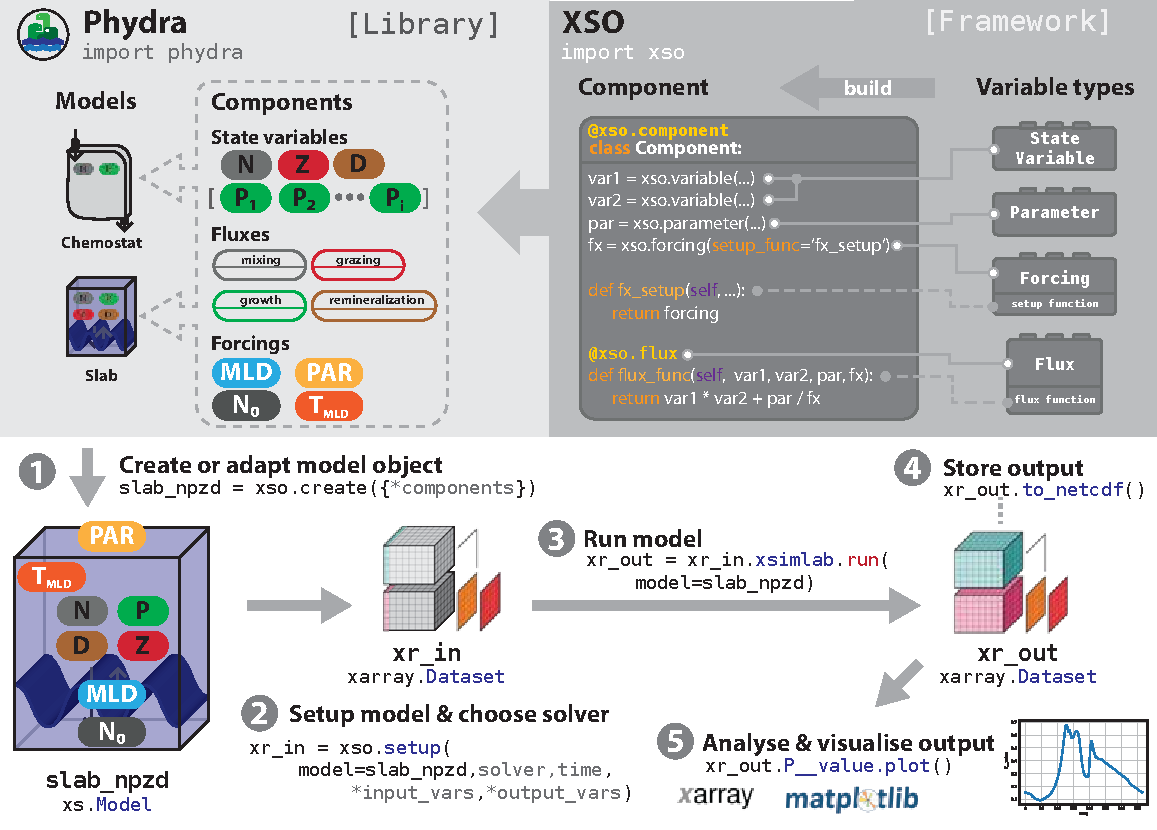
\includegraphics[width=12cm]{Figures/firstdraft_schematics/00_schematics_Package.pdf}
\caption{Schematic of package structure. XSO provides the framework. Phydra is a library of functional \textit{components} and pre-built \textit{model objects}, that can be used, extended and modified. A typical workflow would consist of (1) Choosing a pre-existing model, modifying a model or creating a new model from components. (2) This model has to be setup with the correct labels and parameters, and a solver is chosen. (3) The model can be run efficiently, all input and output data is contained in Xarray datasets (4) that can be conveniently stored or shared. (5) Model output is returned as a "filled-out" Xarray dataset that is fully compatible to be analysed and visualized with the wealth of tools provided by the Python scientific ecosystem. The workflow is presented in further detail in section \ref{Section:ModelDevelopmentWorkflow}.}
\label{Figure:PhydraXSOPackageSchematics}
\end{figure*}

This section illustrates the key steps of configuring and running an ecosystem model using the XSO framework. The workflow is visualized in figure \ref{Figure:PhydraXSOPackageSchematics} and will be further explained below.

\begin{enumerate}
% this needs to be more user workflow, less backend explanation (leave that to previous framework explanation), instead focus on the actual functions and arguments, step by step
    \item \textbf{Creating a \textit{model object}}: 
    A typical modeling workflow would begin with a \textit{model object}. The \textit{model object} can be imported from the Phydra library or assembled from the provided \textit{components}. Creating custom \textit{components} is explained in section \ref{Section:CreatingXSOComponent}.
    To create a \textit{model object}, the function \texttt{xso.model()} is called with a single argument:
    \begin{itemize}
        \item \texttt{model\_dict}: A dictionary of model \textit{components} with their respective labels. The supplied labels identify the \textit{components} for all future steps and allow reusing \textit{components} with unique labels.
    \end{itemize}
    The function call automatically includes processes handling model assembly and the solver backend. When creating a model, the XSO framework automatically orders the processes in their logical order of execution and returns the \textit{model object}. The user can interactively view all parameters required as input at model setup, when printing the object in the console.

    \item \textbf{Creating a \textit{model setup}}: 
    The next step is to create a \textit{model setup} corresponding to the \textit{model object}.
    The \textit{model setup} object is a Xarray dataset that contains all provided parameters as well as the initialized labelled model dimensions and supplied metadata. It is created with a call to \texttt{xso.setup()} by supplying the following arguments:
    \begin{itemize}
        \item \texttt{model}: This argument takes the \textit{model object} created in the previous step. It provides the blueprint for the \textit{model setup} and the backend checks \textit{components} and variabel labels against the provided \textit{model object}.
        \item \texttt{solver}: The solver can be chosen from those implemented in the XSO backend via the appropriate string label. Additionally the user can supply a custom solver implementation based on the abstract solver base class available within the XSO framework.
        \item \texttt{input\_vars}:
        In order to fully initialize a model that can be solved, a user needs to be supply a complete set of parameters and labels linking forcings and variables between \textit{components} to the \texttt{input\_vars} argument. The argument takes a dictionary where each component is referenced via the label supplied when the \textit{model object} was created. The parameters and variables are referenced via the attribute names defined when creating the \textit{component}. Multiple values for a specific parameter can be passed with an additional batch dimension. At model runtime the model can be solved for each set of parameters within the batch dimension.
        \item \texttt{output\_vars}: The user can specify output variables, by default (if no input is provided) all values of variables, forcings and fluxes are stored after model runtime.
        \item \texttt{time}: To specify the time-steps used for model execution, the user has to supply an array of time-steps. This can be easily done using Numpy functions such as \texttt{np.linspace} by providing the desired range and time-steps and passing the resulting array to the \texttt{time} argument.
    \end{itemize}
    At this stage the user can store the fully initialized \textit{model setup} to reuse or modify later, or to share with other users.
    
    \item \textbf{Running model simulations}:
    The \textit{model setup} created in the previous step contains all necessary information needed at model runtime. All that is required of the user is to call the \texttt{xsimlab.run()} method and provide a model object that corresponds to the model setup. The runtime method is provided by the underlying Xarray-simlab framework, of which the following arguments are currently required by XSO:
    \begin{itemize}
        \item \texttt{model}: This argument takes the \textit{model object} created in the first step.
        \item \texttt{batch\_dim}: If defined at model setup, the label of the batch dimension has to be supplied to the \texttt{batch\_dim} argument.
    \end{itemize}
    The method returns model output as a new Xarray dataset, which can be used in the following steps.
    
    \item \textbf{Storing model output}: 
    Simulation inputs and outputs can be kept in memory or saved on disk. Storage of labelled multi-dimensional model output to the NetCDF file format is natively supported by Xarray. The provided \texttt{to\_netcdf()} method stores the full model output including metadata and labeled dimensions to a NetCDF file at the user-specified location. The resulting file contains all metadata (e.g. data source or units) supplied by the user at previous steps and can be easily shared or used for further analysis. 
    
    \item \textbf{Analyzing & visualizing model output}:
    The Xarray dataset created at model runtime is natively compatible with a wealth of packages for data analysis and visualisation from the Python scientific ecosystem. Xarray provides built-in compatibility with the standard plotting library Matplotlib and more advanced data-visualisation tools like Hvplot that make full use of the labelled dimensions for plotting multi-dimensional data. The data for a specific dimension can be extracted to Pandas dataframes (a popular package for data analysis) via the \texttt{to\_dataframes()} method. Specific variables can be indexed and extracted as Numpy arrays via their \textit{component} and variable labels. These methods provide a rich interface and full compatibility with advanced data analysis tools created by the open-source Python community.

\end{enumerate}

- This is exemplary model development workflow, provides multiple steps at which exchange can happen. 
- Currently not all functionality of Xarray-simlab is compatible with XSO backend, but as the project is further developed we are looking to extend functionality.
For documented and practical implementations of this model development workflow see the Jupyter notebooks in the model examples folder of the Phydra library (see code availability section).

\subsection{Creating new components}  \label{Section:CreatingXSOComponent}

To implement ecosystem models beyond those included in the Phydra library, users can build custom \textit{components} from a set of \textit{variable types} provided by the XSO framework. Constructing a \textit{component} is as simple as writing a Python class, except that the framework greatly reduces the necessary boilerplate code (e.g. there is need to define dunder methods such as \texttt{\_\_init\_\_}). The \textit{variable types} can be flexibly combined as attributes and function decorators within a class that is decorated with \texttt{@xso.component}. The decorator converts the class to a functional Xarray-simlab \textit{process} and registers the \textit{variable types} in the XSO backend.

The currently implemented \textit{variable types} in the XSO framework are presented below:
\begin{enumerate}
    \item \textbf{\textit{state variable}}: The class attribute \texttt{xso.variable} registers a time-dependent state variable. The following arguments are available:
    \begin{itemize}
        \item \texttt{foreign}: A binary choice exists between defining the \textit{state variable} at model setup locally within the \textit{component}, or retrieving its value defined in another \textit{component}. This choices is given by the \texttt{foreign} argument available for \textit{state variables} and \textit{forcings}. The benefit to defining \texttt{foreign=True} is that a specific variable can be defined in a single component and referenced throughout the model. Additionally the variable can be flexibly modified by exchanging the \textit{component} that defines the referenced \textit{variable type} in the model. When a forcing or state variable defined as \texttt{foreign=False} (the default option) the user needs to supply a string label at model setup that uniquely identifies the variable within the model.
        
        \item \texttt{dims}: A \textit{state variable} can be implemented as a scalar (the default option) or as an array by supplying a string label for the \texttt{dim} argument. The label defines the variable dimension across the model at model setup and runtime.
        
        \item \texttt{list\_input}: XSO implements this feature to allow greater flexibility in setting up components that act on multiple variables in a similar manner. The list input feature can be activated via \texttt{list\_input = True} if the \textit{state variable} is defined as \texttt{foreign = True}. At model setup the user can supply a list of labels that are iterated over, calculating the specific flux acting on each supplied \textit{state variable}.
        
        \item \texttt{flux}: To define a specific mathematical function acting on the \textit{state variable}, a \textit{flux} function needs to be defined within the \textit{component}. Additionally, to create an implicit link between the defined \textit{state variable} and the \textit{flux}, the name of the \textit{flux} function is supplied to the \texttt{flux} argument.
        
        \item \texttt{negative}: If an argument was made to \texttt{flux}, the \texttt{negative} argument allows changing the mathematical sign of how the \textit{flux} affects the \textit{state variable}. The default is that the result of the \textit{flux} is added to the \textit{state variable}. If \texttt{negative=True}, the \textit{flux} will be subtracted.
        
        \item \texttt{groups}: The \texttt{groups} argument takes a string label that can be referenced in a \textit{group} variable in another \textit{component}. The \textit{group} variable assembles all \textit{state variables} (or \textit{forcings} and \textit{fluxes}) that share the same label across the model and can be used as an array of these values. This allows great flexibility in linking variables between \textit{components} to extend or refactor model processes.
        
        \item \texttt{description}: The argument allows passing a short string descriptor of the implemented variable that is included in the \textit{model object}, e.g. to clarifiy the purpose of the variable to a user. The description is available at all steps of the modeling workflow.
        
        \item \texttt{attrs}: The argument allows including more detailed metadata (e.g. units or citation) that will be included with the \textit{model setup} and model output Xarray datasets.
    \end{itemize}
    
    A \textit{component} can contain any number of \textit{state variables}. In the Phydra library we followed the design pattern that \textit{state variables} are defined within a simple \textit{component} that is reused with unique labels for each required variable. All other \textit{components} reference these \textit{state variables} via the \texttt{foreign=True} functionality.
    
    
    \item \textbf{\textit{forcing}}: The class attribute \texttt{xso.forcing} registers an external time-varying parameter. It shares the \texttt{foreign}, \texttt{dims}, \texttt{groups}, \texttt{description} and \texttt{attrs} arguments with the \textit{state variable} attribute. Additionally a forcing needs to be supplied with the following argument:
    \begin{itemize}
        \item \texttt{setup\_func}: The argument has to be supplied with the name of a locally defined forcing setup function. This is a Python function defined within the \textit{component} that contains any necessary logic or computation for supplying the time-dependent forcing to the XSO backend. The setup function constructs and returns the actual forcing function, that takes model time as input and returns the value of the forcing during model runtime.
    \end{itemize}
    
    Constant forcings could be supplied via a single parameter to a \textit{flux}, but in the Phydra library constant forcings are generally implemented as \textit{forcing} variables, to allow easy exchange to variable forcings without having to modify other \textit{components} in model. 

    All variables and parameters defined within component can be used as arguments in both the setup function and the forcing function, e.g. to calculate station-specific forcing from a more general \textit{component}.
    
    If the forcing is based on data and not a mathematical function or constant value, it is necessary to perform some type of interpolation to supply the forcing to the model at flexible time steps. The interpolation would naturally happen within the setup function, where the choice of interpolation algorithm is up to the user. In Phydra we use \texttt{scipy.interpolate.splrep}, an algorithm to calculate the B-spline representation of a 1-D curve, in particular because it allows for periodic interpolation that is useful for yearly climatological forcing.
    
    \item \textbf{\textit{parameter}}: 
    Model parameters can be added to a \textit{component} via the \texttt{xso.parameter} class attribute. It shares the \texttt{dims}, \texttt{description} and \texttt{attrs} arguments with the \textit{state variable} attribute. Any parameter defined as an attribute is available as an argument to the \textit{flux} and forcing setup functions within a \textit{component}. The specific value of the \textit{parameter} is supplied at model setup.
    
    \item \textbf{\textit{group}}: Class attribute
    The \texttt{xso.group} class attribute allows creating a \textit{group variable} that aggregates multiple variables defined in other components. \textit{State variables}, \textit{forcings} and \textit{fluxes} provide a \texttt{groups} argument that can be supplied with a string label. By supplying the same string label to the \texttt{name} argument of the \textit{group} variable, all variables defined in other components that match the label are collected as a list. 
    This group variable can be used in the calculation of fluxes similar to any other locally defined \textit{variable type} within the same \textit{component}. This allows for flexibility in model setup and provides extensible of models, e.g. growth-limiting terms can be aggregated to a final component that calculates total flux and limiting terms can removed or added flexibly.
    
    \item \textbf{\textit{flux}}: 
    The previous building blocks for state variables, forcings and parameters create the structure of the model, but when solved at this stage there would be no meaningful simulation. The basic building block of the system of differential equations that underpin an XSO model are \textit{fluxes}. A \textit{flux} is a Python function within a \textit{component} that takes the locally defined \textit{state variables}, \textit{forcings} and \textit{parameters} as input arguments and is decorated with \texttt{@xso.flux}. The decorator can be used as is or supplied with specific values for the \texttt{dims}, \texttt{groups}, \texttt{description} and \texttt{attrs} arguments. The \textit{flux} defines a mathematical function acting on state variables that can be directly linked to a \textit{state variable} via their \texttt{flux} argument or can be passed along to a \textit{group} variable and assigned to a \textit{state variable} in another \textit{component}.

    
\end{enumerate}

A \textit{component} can contain any number of \textit{variable types} as attributes, as well as helper functions or other custom attributes and methods. A complex flux can be broken down into multiple functions contained in the same decorated Python class.

- Components do not rely on inheritance, which improves code readability and maintainability. Due to the decorating function and translation process, backend is highly flexible and hides complexity from users who want to focus on the scientific questions. But as an open-source project, more advanced users can delve into the backend that can be modified for custom applications.


 %% \ SECTION 3
\section{Model use cases} \label{Section:UseCases}

To showcase the utility of Phydra, we present three model use cases of varying complexity. Per use case, we present model description and formulations, as well as the implementation within the XSO framework and exemplary model results. As part of the implementation we show a modification to each model that highlights the modular nature of the framework.

The three models and all their components are included within the first release of the Phydra library. Users could start experimenting with the existing models or assemble their own from the included components, as all included components were designed to be compatible within the library. In future versions of Phydra, these models will be extended, and many other model structures could be added as the user base grows.

For the first use case, a simple chemostat model, we present the full implementation with XSO variable types within the components. To simplify the presentation of the more complex models in use cases 2 and 3, we show only the component structure and highlight additional technical aspects of the technical implementation. For all use cases the complete code, following the full model development workflow from model creation to output visualisation is available publicly as interactive Jupyter notebooks in the Phydra repository (\url{https://github.com/ben1post/phydra/tree/master/examples}).

\subsection{Model use case 1: Phytoplankton growth in a chemostat}

%%f
\begin{figure}[t]
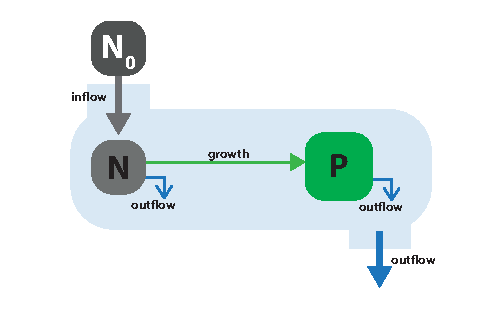
\includegraphics[width=8.3cm]{Figures/firstdraft_schematics/01_schematics_Chemostat.pdf}
\caption{Model schematic for use case 1: Monod model of phytoplankton feeding on a single nutrient in a flow-through system. Light blue shape represents model system, with an external nutrient medium with concentration $N0$ flowing into $N$, which is in turn taken up by $P$. Both $N$ and $P$ flow out at a constant rate and the modeled volume remains constant.}
\label{Figure:ModelSchematics_1}
\end{figure}

Chemostats are a commonly used experimental setup for studying the dynamics of planktonic microorganisms under controlled laboratory settings. With a constant influx of medium containing nutrients that is matched by a constant outflow rate of the medium from the system, scientists can grow microorganisms under constant abiotic conditions. Seminal advancements in the study of marine ecosystems, in particular the mechanisms and dynamics of phytoplankton growth, were made by scientists using chemostats \citep[e.g.,][]{Droop1968VitaminLutheri}. Although chemostat systems are not commonly found in nature, some oceanic upwelling systems can be approximated with such a simple model \citep{Haefner2005ModelingApplications}.

We chose a chemostat setting for the first use case model, due to the relatively simple mathematics that can describe such a flow-through system. It lends itself well as a test-bed for complex ecosystem model formulations. The presented model is a very simple construct, of a single phytoplankton state variable growing on a single nutrient with Monod kinetics. The Monod model, devised to describe bacterial growth, assumes that phytoplankton growth rate is proportional to the nutrient uptake rate \citep{Monod1942RecherchesBacteriennes}.
It is the canonical formulation used in most marine ecosystem models to this day, although it is not without caveats \citep{Hellweger2017a}. More complex treatments of growth have been developed, most notably the Droop model \citep[e.g.,][]{Droop1968VitaminLutheri}, however we chose to present the simplest possible ecosystem formulation to present the technical framework employed in the Phydra library.

To showcase the flexibility of using the XSO framework, we show the simplicity of adding a different forcing, here a sinusoidal varying nutrient concentration in the supplied medium.

\subsubsection{Description}
The model is schematized in Figure \ref{Figure:ModelSchematics_1}. It uses nitrogen as its currency (quantities are measured in units of $\mu mol$ N $m^{-3}$, or $\mu M$), with state variables for dissolved nutrients ($N$) and phytoplankton ($P$). The physical environment is a highly simplified flow-through system, corresponding to a laboratory chemostat setup. Growth medium with nutrient concentration $N_0$ flows into the system at rate $f$. The model components ($N$ \& $P$) flow out of the system at that same rate.

Nutrient limitation of phytoplankton growth ($\gamma$) is described via Monod kinetics \citep{Monod1942RecherchesBacteriennes}.
\begin{equation}
    \gamma = \frac{N}{k + N} 
\end{equation}
where $k$ is the half-saturation constant. $N$ is ambient nutrient concentration in the medium.
The realized growth rate is a product of the nutrient-limiting term $\gamma$ and the maximum growth rate $\mu_{max}$.
Pathways relating to detrital matter, mortality and regeneration are not resolved. 

The model equations are as follows:
\begin{equation}
    \frac{d N}{d t} = 
    f N_0 % Nutrient mixing
    -  \mu_{max} \frac{N}{k_N + N} 
    - f N
\end{equation}

%PHYTOPLANKTON
\begin{equation}
    \frac{d P}{d t} =
    \mu_{max} \frac{N}{k_N + N} 
    - f P
\end{equation}


\subsubsection{Implementation}

%%f
\begin{figure*}[t]
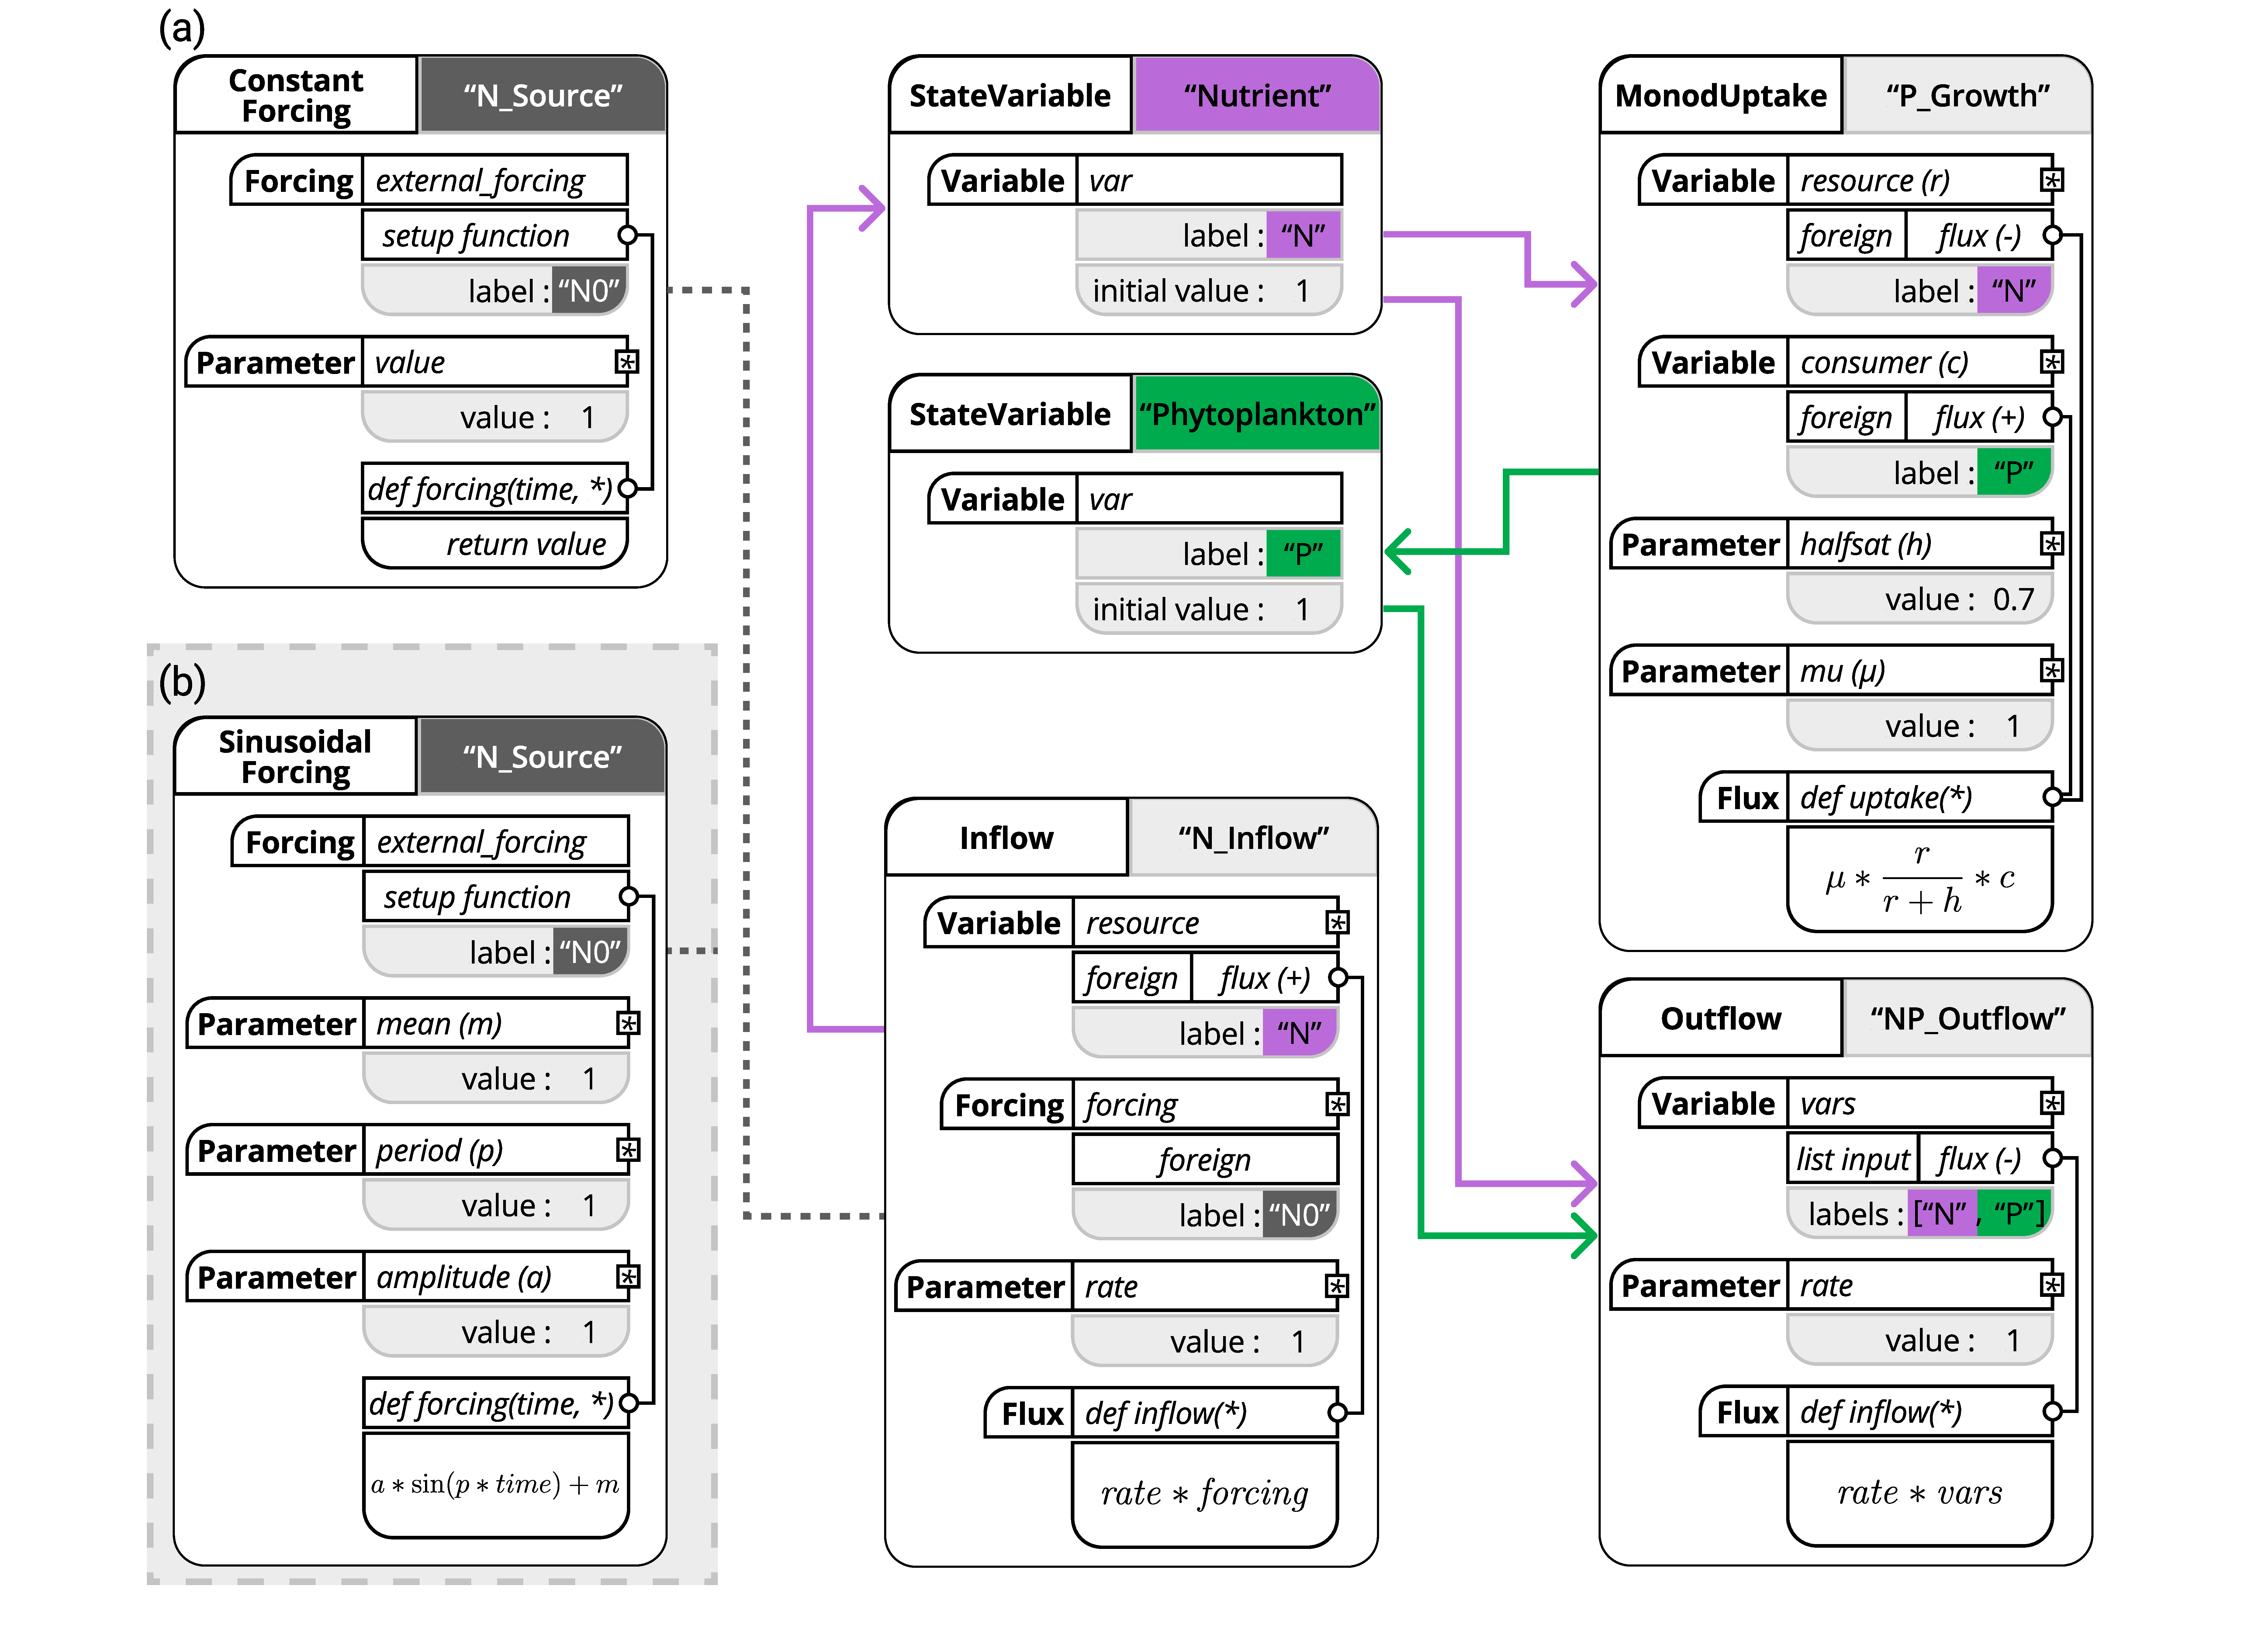
\includegraphics[width=15cm]{Figures/firstdraft_schematics/code_schematics/Chemostat.pdf}
\caption{Schematic of use case 1 model as implemented in the XSO framework and included in the Phydra library. (a) shows model setup under constant forcing, (b) shows the forcing component supplying sinusoidal forcing. Structures in solid black are hard-coded into components. Labels of the different components are supplied at model creation, while gray boxes and the resulting linkages between components (shown in thick colored arrows and dashed lines) are defined at model setup, via the supplied labels and parameters. The asterisk in the flux function input arguments references the variables, forcings and parameters defined within the same component, these local variables can be used in all functions (e.g. fluxes or forcing setup functions) within that same component.}
\label{Figure:CodeSchematics_1}
\end{figure*}

The chemostat model was implemented using the XSO framework. In order to find a useful structuring of model components, we can separate the model into state variables, forcings and fluxes. For state variables we have the nutrient ($N$) and phytoplankton ($P$). The only forcing is the nutrient concentration of the external medium ($N_0$). Three fluxes can be separately defined: The inflow of the external medium, $P$ growing on $N$ and the outflow of both $N$ and $P$.
The model was implemented using these 6 separate model components as visualized in Figure \ref{Figure:CodeSchematics_1}.

We start model construction from the list of state variables, forcings and fluxes mentioned before. Below we list the model components with a short explanation to their functionality and go through the XSO variable types used within:
\begin{enumerate}
    \item \texttt{StateVariable} defines a state variable locally within the component, and is implemented twice, for nutrient and phytoplankton respectively.
    \begin{itemize}
        \item \texttt{var}: A \texttt{xso.variable} that registers the state variable at model creation. At model setup the variable requires two inputs: The specific label used throughout the model to reference this state variable in other components and the initial value of this state variable.
    \end{itemize}
    
    \item \texttt{ConstantForcing} creates and registers a constant forcing value, that can be referenced in other components. Here it is employed to create the forcing for the nutrient concentration ($N_0$).
    \begin{itemize}
        \item \texttt{forcing}: A \texttt{xso.forcing} that registers the forcing at model creation. The variable has to be initialized with a setup function within the same component. At model setup the specific forcing label used in the model has to be supplied ("N0" in this case).
        \item \texttt{rate}: A \texttt{xso.parameter} whose value is supplied at model setup and is used within the forcing setup function.
        \item \texttt{def forcing(time,*)}: This is a basic Python function defined within the component class, that is linked via its name to the forcing variable defined above. The asterisk is pseudo-code to reference the availability of all parameters defined in the component, specifically the \texttt{rate} parameter defined above. The setup function can include code to read or modify data, or calculate a specific time-dependent forcing. This forcing is then registered in the XSO framework, and will be called within the model backend when the forcing is referenced in other components.
    \end{itemize}
    
    \item \texttt{Inflow} is our first component that defines a flux, in this case the constant input of medium with nutrient concentration $N_0$ into our medium.
    \begin{itemize}
        \item \texttt{resource}: A \texttt{xso.variable} with the argument \texttt{foreign=True}. At model setup this variable requires a single input, which is the label of the state variable that should be affected by the fluxes defined in the component. The other arguments that are necessary for this is \texttt{flux="inflow"}, referencing the flux defined below. By default the flux is adding to the state variable, but this can be modified by passing the argument \texttt{negative=True} if so required.
        \item \texttt{forcing}: A \texttt{xso.forcing} with the argument \texttt{foreign=True}. Similar to the variable defined above, this forcing requires a label to the foreign forcing referenced here. It can be used as an argument in the flux function defined below.
        \item \texttt{rate}: A \texttt{xso.parameter} whose value is supplied at model setup and is used within the flux function below.
        \item \texttt{def inflow(*)}: A basic Python function decorated with \texttt{@xso.flux}. Through the flux argument supplied to \texttt{resource} it is linked via its name to the foreign state variable. The asterisk is pseudo-code to reference the availability of all parameters and forcings defined within the component, specifically we use the \texttt{rate} parameter and \texttt{forcing} defined above. This flux function consists of the basic mathematical calculation that defines the flux. For this simple constant input it calculates \texttt{forcing * rate} and adds that value to the state variable \texttt{resource}. With the labels and values supplied at model setup this flux returns $N_0 * 0.1$ at model runtime.
    \end{itemize}
    
    \item \texttt{MonodGrowth} is another component that defines a flux, in this case the uptake of nutrient and growth of phytoplankton based on Monod kinetics.
    \begin{itemize}
        \item \texttt{resource}: A \texttt{xso.variable} with the argument \texttt{foreign=True}. The flux \texttt{"uptake"} is linked via the \texttt{flux} argument with the option \texttt{negative=True} enabled. At model setup we supply the label \texttt{"N"}.
        \item \texttt{consumer}: A \texttt{xso.variable} with the argument \texttt{foreign=True}. The flux \texttt{"uptake"} is linked via the \texttt{flux} argument. At model setup we supply the label \texttt{"P"}.
        \item \texttt{halfsat}: A \texttt{xso.parameter} defining the half-saturation constant whose value is supplied at model setup and is used within the flux function below.
        \item \texttt{mu}: A \texttt{xso.parameter} defining the phytoplankton growth rate whose value is supplied at model setup and is used within the flux function below.
        \item \texttt{def uptake(*)}: This is Python function  decorated with \texttt{@xso.flux}. It is linked to the state variable defined as \texttt{resource} as negative term, and adds to the total flux of the state variable defined as \texttt{consumer} at model setup. The flux function returns a Monod function based on the values of \texttt{resource} and \texttt{consumer}, as well as the parameters \texttt{halfsat} and \texttt{mu} in the mathematical formulation $\mathit{mu} \frac{\mathit{resource}}{\mathit{halfsat}+\mathit{resource}} \mathit{consumer}$. With the labels supplied at model setup it returns $\mu \frac{N}{k_N+N} P$.
    \end{itemize}
    
    \item \texttt{Outflow} is final component defining a flux, specifically the outflow of both $N$ and $P$.
        \begin{itemize}
        \item \texttt{vars}: A \texttt{xso.variable} with the arguments \texttt{foreign=True} and \texttt{list\_input=True}. The flux is linked via \texttt{flux="outflow"} with the optional argument \texttt{negative=True} enabled. At model setup this variable requires a single input, which is a list of the labels of the state variables that are be affected by the flux defined in the component. Here we supply \texttt{["N","P"]}.
        \item \texttt{rate}: A \texttt{xso.parameter} whose value is supplied at model setup and is used within the flux function below.
        \item \texttt{def outflow(*)}: A basic Python function decorated with \texttt{@xso.flux}. The defined flux is computed individually for all state variables supplied to \texttt{vars}, but can be coded as a simple mathematical function with the framework handling the necessary routing. For this simple flux it calculates \texttt{vars * rate} and substracts that value from the state variables. With the labels and values supplied at model setup this flux returns $- N * 0.1$ acting on $N$ and $-P * 0.1$ acting on $P$ at model runtime.
    \end{itemize}
\end{enumerate}

The \texttt{Outflux} component shows off a feature of XSO, where fluxes affecting multiple variables in the same way allow for the definition of a list input to the variable at model setup. The flux function is computed for each supplied label in the list, and the XSO framework handles the routing of the flux values to their respective state variable. Particularly for models including many state variables, this feature simplifies the model creation and setup steps.

%%% TWO-COLUMN TABLE
%
%t
\begin{table*}[t]
\caption{Model parameters used in runs for use case 1:}
\begin{tabular}{l c c r}
\tophline
Parameter & Description & Value & Units \\
\middlehline

$\mu_{max}$ & maximum growth rate & 1 & \unit{d^{-1}} \\
$f$ & flow rate & 0.1 & \unit{d^{-1}}\\
$k$ & half-saturation constant for nutrient uptake & 0.7 & \unit{µM \ N}\\

\bottomhline
\end{tabular}
\belowtable{These exemplary parameters are not representative for a natural system} % Table Footnotes
\label{Table:UseCase1Parameters}
\end{table*}
%

To explore the basic dynamics, we chose parameters arbitrarily from standard ranges for exemplary model runs. See table \ref{Table:UseCase1Parameters} for the specific parameters values used. Initial values for the state variables $N$ and $P$ where set at 1 and 0.1 respectively. A more profound analysis would require testing parameter ranges, but for the simple demonstration we aim at here this should suffice.

Also shown in Figure \ref{Figure:CodeSchematics_1} is the component that was used to modify the model from a system under constant forcing to periodic forcing. In order to run this model at periodic forcing we can simply exchange the Forcing component, from \texttt{ConstantForcing} to \texttt{SinusoidalForcing}. This specific component requires more input parameters, but otherwise the model creation and setup steps remain exactly the same. In fact there is the option to update the pre-existing model object and model setup object by simply supplying the \texttt{SinusoidalForcing} component for the \texttt{"N\_inflow"} component via the \texttt{model.update\_processes()} method and updating the corresponding parameters via \texttt{model\_setup.update\_vars()} functions supplied by the Xarray-Simlab framework that XSO extends. Such functionality allows straightforward modification and testing of models.

\subsubsection{Results}

%%f
\begin{figure}[t]
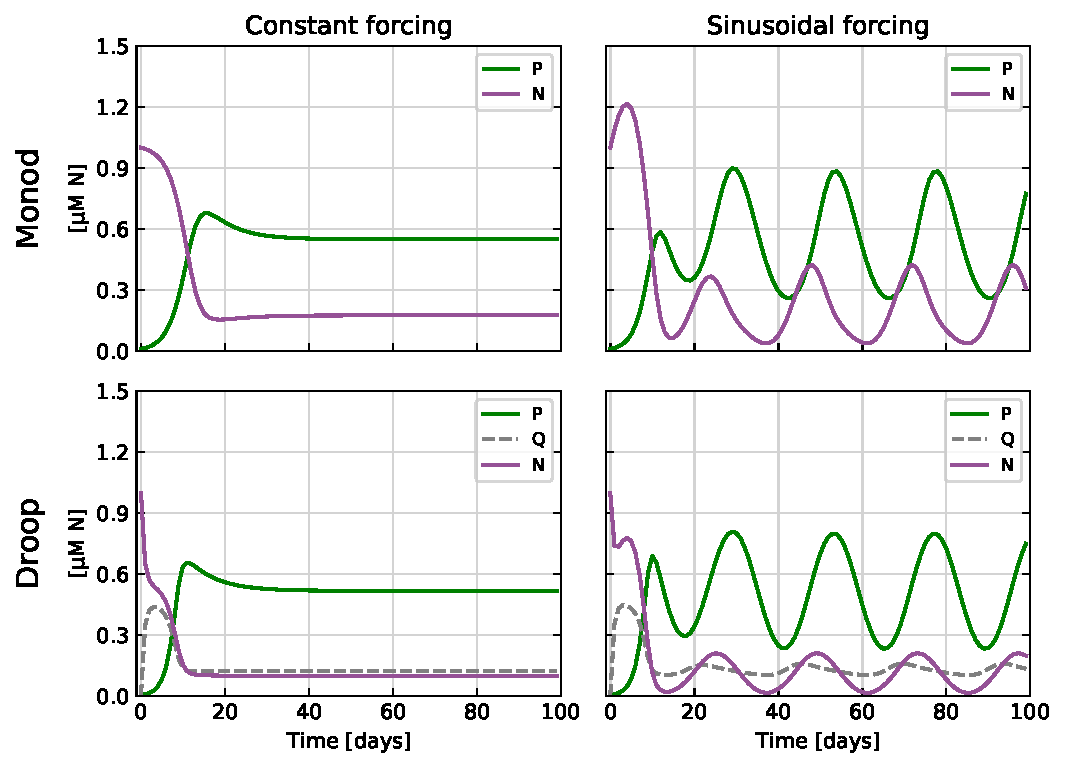
\includegraphics[width=8.3cm]{Figures/firstdraft_plots/01_chemostat_output.pdf}
\caption{Model output for the four chemostat model scenarios. (a) Constant forcing, (b) Sinusoidal forcing}
\label{Figure:ResultsChemostat}
\end{figure}

For the two model runs, one with a nutrient medium with constant nutrient concentration and the other with periodically variable nutrient concentration, the time series for both $N$ and $P$ are shown in Figure \ref{Figure:chemostat_plot}.
For the constant forcing scheme, the model quickly reaches a steady state, as nutrient supply and the resulting phytoplankton growth balances with the loss of nutrient and phytoplankton due to the constant outflux of medium.
The periodically variable nutrient concentration drives a similarly variable phytoplankton concentration, after a short initial growth burst. The resulting oscillations center around the same value (0.9 \unit{µM \ N}) that the phytoplankton population reached under the constant scheme. This is to be expected due to the nutrient supply being centered around the same mean value (1 \unit{µM \ N} for both schemes).

The oscillations show a similar pattern to predator-prey models (e.g. Lotka-Volterra), however in this model this is fully driven by our external forcing and not due to feedback mechanisms within the ecosystem model. Phytoplankton growth fully utilizes surplus nutrients subsequently depletes the falling nutrient concentration. In contrast, the constant model shows no depletion of nutrients as the phytoplankton population can not exceed nutrient supply with our chosen parameters.

Our first use case represents a basic proof-of-concept that our presented library and framework can create expected results with a very simple model setup. The exchange of the forcing component highlights the modularity of the XSO framework. This simple chemostat model provides a template for users to start experimenting from.

\subsection{Model use case 2: An NPZD slab model - EMPOWER}
%%f
\begin{figure}[t]
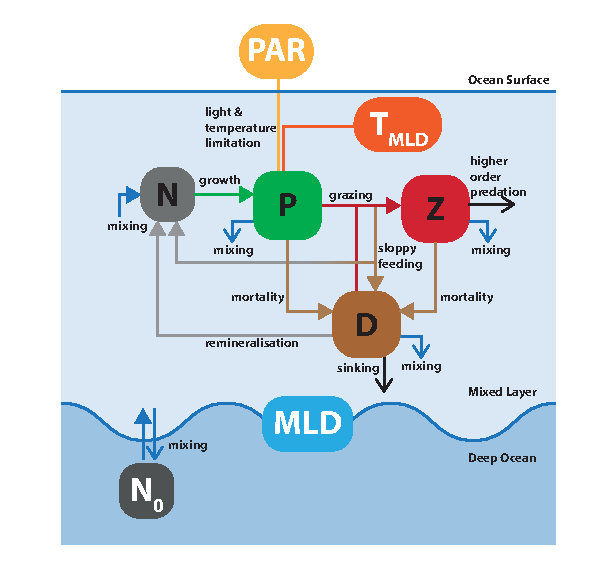
\includegraphics[width=8.3cm]{Figures/firstdraft_schematics/02_schematics_EMPOWER.pdf}
\caption{Model schematic of NPZD slab model presented as the second use case. Model structure is adapted
from \citet{Anderson2015c}. Boxes with black font represents state variables, while boxes with white font represent external forcings. Arrows indicate fluxes between state variables, with line arrows representing loss fluxes from the model system. The upper layer box contains the ecosystem model. The curvy line represents the variable mixed layer depth that defines the boundary to the inert deep ocean.}
\label{Figure:ModelSchematics_2}
\end{figure}

Our second use case presents a classical NPZD model embedded in a slab-ocean physical setting, as originated by \citet{Steele1962EnvironmentalSea}. The simplified two-layer structure provides a zero-dimensional and mechanistically simple description of physical processes affecting euphotic ecosystems in the open ocean. Major advancements in computational descriptions of our oceans were made using this setup \citep[e.g.,][]{Evans1985ACycles, Fasham1990a} The classical structure lends itself well as an efficient physical test-bed for more complicated ecosystem descriptions and is often used as a teaching example as an entry point into marine ecosystem modeling \citep{Anderson2015c}.
The presented model is an implementation of the elegant EMPOWER model, as presented by \citet{Anderson2015c}. See Figure \ref{Figure:ModelSchematics_2} for a schematic of the model structure.

The published model code was written as an R script, with some modifications allowed via user supplied flags. We updated the model code to the modular and flexible XSO framework, allowing for greater adaptability and experimentation on this classical structure.

Many NPZD-type models have been published over the years with a plethora of different formulations for the functional responses of the ecosystem components. The EMPOWER model was presented with various formulations for the treatment of light, and we followed this path by showing two different light-attenuation algorithms that can be easily exchanged in the modular framework. 

\subsubsection{Description}
% really present a concise and to the point model description here, as would be in any other model publication.
For the second use case we have implemented a traditional NPZD ecosystem model as presented in Figure \ref{Figure:ModelSchematics_2}. It uses nitrogen as its currency (quantities are measured in units of $\mu mol$ N $m^{-3}$, or $\mu M$), with state variables for dissolved nutrients ($N$) and phytoplankton ($P$), zooplankton ($Z$) and detritus ($D$). The model employs slab physics as presented in \citet{Evans1985ACycles}. The model ocean is built up of two layers. A biologically inert deep ocean is situated below a well mixed upper layer of variable depth that contains the ecosystem. The model structure, locations and parameters are adapted from the EMPOWER model presented by \citet{Anderson2015c}.

The model is driven by empirical forcing describing the depth of the mixed layer ($H$), average temperature of the mixed layer ($T$), photosynthetically active radiation at the surface ($I$) and nutrient concentration in the deep layer ($N_0$) 

% Nutrient dynamics
The zero-dimensional slab setting describes two vertical layers of which the deeper layer supplies nutrients to the upper layer, whilst other components are mixed to the deep layer and lost from the system.
The magnitude of mixing is described by the coefficient $K$:

\begin{equation}
    K = \frac{h^{+} + \kappa}{H}
\end{equation}

Constant diffusive mixing is parameterized by $\kappa$. Variable mixing is a function of the change in mixed layer depth (MLD) over time $h = \frac{d}{d t} H$. The derivative of MLD ($h$) is positive when the mixed layer deepens. The function $h^{+}$ defines the effects of entrainment and detrainment due to the changes in MLD as $h^{+} = \max(0, \ h)$. When the mixed layer shallows, $h^{+}$ does not modify $K$ (i.e. returns 0 instead of a negative value), based on the assumption that detrainment of mass and the increase in concentration due to the reduced volume of the mixed layer are balanced \citep{Evans1985ACycles}. 

%\subsubsection{Nutrients}
Dissolved inorganic nitrogen in the mixed layer ($N$) is supplied via mixing, zooplankton excretion and detritus remineralisation.
Nutrients are entrained from the bottom layer. Mixing of nutrients is a positive term adding to $N$ along the gradient between $N_0$ and $N$. The general direction of transport is from a nutrient-rich bottom layer to the upper layer supporting phytoplankton growth, which is the only loss term for $N$.

%\subsubsection{Phytoplankton}
Phytoplankton biomass ($P$) increases through temperature-dependent, light- and nutrient-limited growth. The growth rate ($\mu_{P}$) is the product of a temperature-dependent maximum growth rate ($\mu_P^{max}(T)$) and the growth-dependencies on light ($\gamma^{I}$) and nutrients ($\gamma^{N}$): 

\begin{equation}
    \mu_{P} = \mu_P^{max}(T) \ \gamma^{I} \ \gamma^{N}
\end{equation}

$T$ is the average temperature of the mixed layer in \unit{\degree C}, as supplied from model forcing. Under the assumption of balance growth, the maximum growth rate of phytoplankton $\mu_P^{max}(T)$ is equivalent to the temperature-dependent maximum photosynthetic rate $V_P^{max}(T)$. Temperature dependence is calculated via the Eppley curve \citep{Eppley1972TemperatureSea}, with an exponential equivalent to a $Q_{10}$ of 1.895.

\begin{equation}
    V_P^{max}(T) = V_P^{max}(0) \ 1.066^T
\end{equation}

Nutrient limitation of phytoplankton growth $\gamma^N$ is described by the Michaelis-Menten (or Monod) equation.

\begin{equation}
    \gamma^N = \frac{N}{k_N + N}
\end{equation}

where $k_N$ is the half-saturation constant for nutrient uptake. $N$ is the ambient nutrient concentration, in this case of dissolved inorganic nitrogen (DIN). In this simple model there is no distinction between nutrient uptake and assimilation of nutrient via growth.

The light-limiting term $\gamma_{I}$ represents growth-dependence on total light ($I$) available to phytoplankton the upper mixed layer. We use Smith's formulation to calculate the photosynthetic rate of phytoplankton dependent on irradiance.

\begin{equation}
    V_P = \frac{\alpha ~ I ~ V_P^{max}}{\sqrt{(V_P^{max})^2 + \alpha^2 I^2}}
\end{equation}

Where $V_P^{max}$ is the maximum photosynthetic rage, $\alpha$ is the slope of the PI curve and $I$ is irradiance.

Attenuation of $I$ at depth $z$ in the mixed layer is calculated according to the Lambert-Beer equation:

\begin{equation}
    I(z) = I \ \exp{(-k_{PAR} \ z)}
\end{equation}

The attenuation coefficient $k_{PAR}$ is the sum of the attenuation coefficient of seawater $k_w$ and that of phytoplankton biomass $k_c$, which is multiplied by the current phytoplankton biomass $P$:

\begin{equation}
    k_{PAR} = k_w + k_c \cdot P
\end{equation}

Combining the equations and integrating across the mixed layer, the numerical solution for the integrated light-limiting term affecting phytoplankton growth is calculated.
% Perhaps show fully integrated equation in appendix?

The modification we show here calculates light attenuation for a three-layer model of the mixed layer, as developed by \citet{Anderson1993APhotosynthesis}. This formulation calculates multiple $k_{PAR, i}$, with i = 1 for the top 5 \unit{m}, i = 2 for the depth range 5 - 23 \unit{m} and i = 3 for depths below 23 \unit{m}. The changing spectral properties of water are taken into account via polynomial coefficients ($b_{0,i}$ to $b_{5,i}$).
\begin{equation}
    k_{PAR, i} = b_{0,i} + b_{1,i} C^{1/2} + b_{2,i} C + b_{3,i} C^{3/2} + b_{4,i} C^2 + b_{5,i} C^{5/2}
\end{equation}
where $C$ represents the pigment (chlorophyll) concentration. The values of the polynomial coefficients are given in the appendix.

See \citet{Anderson2015c} for further discussion of the used formulations and a more in-depth presentation of light-limitation formulations.

Non-grazing mortality of phytoplankton is described by both a linear $m_P$ and a quadratic factor $m_{P2}$ \citep{Yool2011Medusa-1.0:Domain}. The former accounts for natural mortality and excretion. Quadratic mortality describes density-dependent loss processes, which can be caused by viral infection. All non-grazing phytoplankton loss terms feed into the detritus pool.

%\subsubsection{Zooplankton}
Grazing by zooplankton occurs on both phytoplankton and detritus. The grazing function is a Holling Type 3 grazing response as presented in \citet{Anderson2015c}:

\begin{equation}
    G_P = \mu_Z \left( \frac{ \hat{\varphi}_P P}{(k_Z)^2 + \hat{\varphi}_D D +\hat{\varphi}_P P}  \right) Z
\end{equation}
where $\hat{\varphi}_P$ = $\varphi_P \ P$, $\hat{\varphi}_D$ = $\varphi_D \ D$.

This formulation describes the total biomass of phytoplankton that is grazed $G_P$. Parameter $\mu_Z$ is the maximum ingestion rate for a food source, in this case both phytoplankton and detritus. 
The grazing preference parameters $\varphi_P$ and $\varphi_D$ do not represent a discrete fraction of the amount grazed in the diet relative to the environment. Instead, this amount is represented by the ratio of $\hat{\varphi}_P$ and $\hat{\varphi}_D$. 
The half-saturation constant for grazing $k_Z$ is an arbitrary parameter, that scales the density-dependent half-saturation constant $k_P$ for grazing on phytoplankton based on the choice of $\varphi_P$, with the relationship $k_P$ = $\sqrt{\frac{(k_Z)^2 }{\varphi_P}}$.

Similarly the detritus grazing flux is defined as:
\begin{equation}
    G_D = \mu_Z \left( \frac{ \hat{\varphi}_D D}{(k_Z)^2 + \hat{\varphi}_D D +\hat{\varphi}_P P}  \right) Z
\end{equation}

This sigmoidal response includes passive prey switching via an interference effect, where the increase in biomass of one prey slightly reduces the intake of other prey. In contrast to other grazing formulations \citep[e.g.,][]{Fasham1990a}, the prey switching mechanism does not create sub-optimal feeding, where an increase in biomass of less common prey can decreases the total grazing flux \citep{Gentleman2003a}.

Zooplankton ingestion of prey does not directly convert to biomass gained however. The total biomass grazed ($G_P + G_D$) is split three ways between zooplankton growth (to $Z$), excretion of dissolved nutrients (to $N$) and egestion of faecal matter \& particles (to $D$). Zooplankton growth is a product of total biomass grazed ($G_P$) and the gross growth efficiency (GGE) of zooplankton. The two parameters defining GGE in this model are absorption efficiency ($\beta$) and net production efficiency ($\epsilon$). Adsorption efficiency $\beta$ describes the fraction of $G_P$ which is absorbed in the gut, of which the fraction $\epsilon$ is actually assimilated into biomass (to $Z$: \ $\beta \epsilon$), while the rest is excreted as DIN (to $N$: \ $\beta (1-\epsilon)$). GGE specifically is the product of $\epsilon$ and $\beta$, for which values between 0.2 and 0.3 have been observed for a wide range of zooplankton \citep{Straile1997GrossGroup}. The fraction of $G_P$ egested to $D$ (e.g. as faecal pellets) is calculated via $1-\beta$. 

Similar to phytoplankton mortality, the linear mortality factor $m_Z$ parameterizes natural mortality and excretion and feeds into the pool of detritus. The quadratic factor $m_{Z2}$ describes higher order predation on zooplankton and is removed from the system. 

%\subsubsection{Detritus}
Detritus concentration in the upper layer ($D$) is supplied by all mortality of phytoplankton, linear zooplankton mortality and zooplankton egestion (e.g. faecal pellets). The loss terms are remineralisation, zooplankton grazing, mixing and an additional sinking flux. 

Detritus is remineralised at a constant rate $m_D$ to $N$. Similar to $P$ and $Z$, $D$ is affected by mixing through changes in MLD, described by the mixing coefficient $K$. In addition to $K$, detritus experiences losses due to gravitational sinking at a rate of $v_D$. This term is added to describe the fast export of larger detritus particles below the mixed layer. 

%\subsubsection{Model equations}
The rates of change of the state variables are described by the following set of equations. For the definition of all symbols used here see Table \ref{appendix:table:usecase1symbols}. See \citet{Anderson2015c} for a more detailed discussion of model structure and formulation.

%Nutrient
\begin{equation}
    \frac{d N}{d t} = 
    K (N_0 - N) % Nutrient mixing
    + \beta(1 - \epsilon)(G_P + G_D) % Unassimilated grazing by Z
    + m_D \ D % Remineralisation of D
    - \mu_{P} \ P % Phytoplankton gains
\end{equation}

%PHYTOPLANKTON
\begin{equation}
    \frac{d P}{d t} =
    \mu_{P} \ P  % Phytoplankton gains
    - m_P \ P % Linear mortality
    - m_{P2} \ (P)^2 % Quadratic mortality
    - G_P % Z grazing
    - K \ P % Phytoplankton mixing
\end{equation}

%ZOOPLANKTON
\begin{equation}
    \frac{d Z}{d t} =
    \beta \ \epsilon(G_P + G_D) % Assimilated grazing
    - m_Z \ Z % Linear mortality
    - m_{Z2} \ (Z)^2 % Quadratic mortality
    - K \ Z % Zooplankton mixing
\end{equation}

%DETRITUS
\begin{equation}
    \frac{d D}{d t} = 
    m_P \ P % Linear mortality
    + m_{P2} \ (P)^2 % Quadratic mortality
    + m_Z \ Z % Linear mortality
    + (1 - \beta)(G_P + G_D) % Unassimilated grazing by Z
    - G_D % Z grazing on D
    - m_D \ D % Remineralisation of D
    - K \ D % Mixing of D
    - \frac{v_D}{H} \ D % Sinking of D
\end{equation}


\subsubsection{Implementation}
% here present the implementation as is used in phydra

%%f
\begin{figure*}[t]
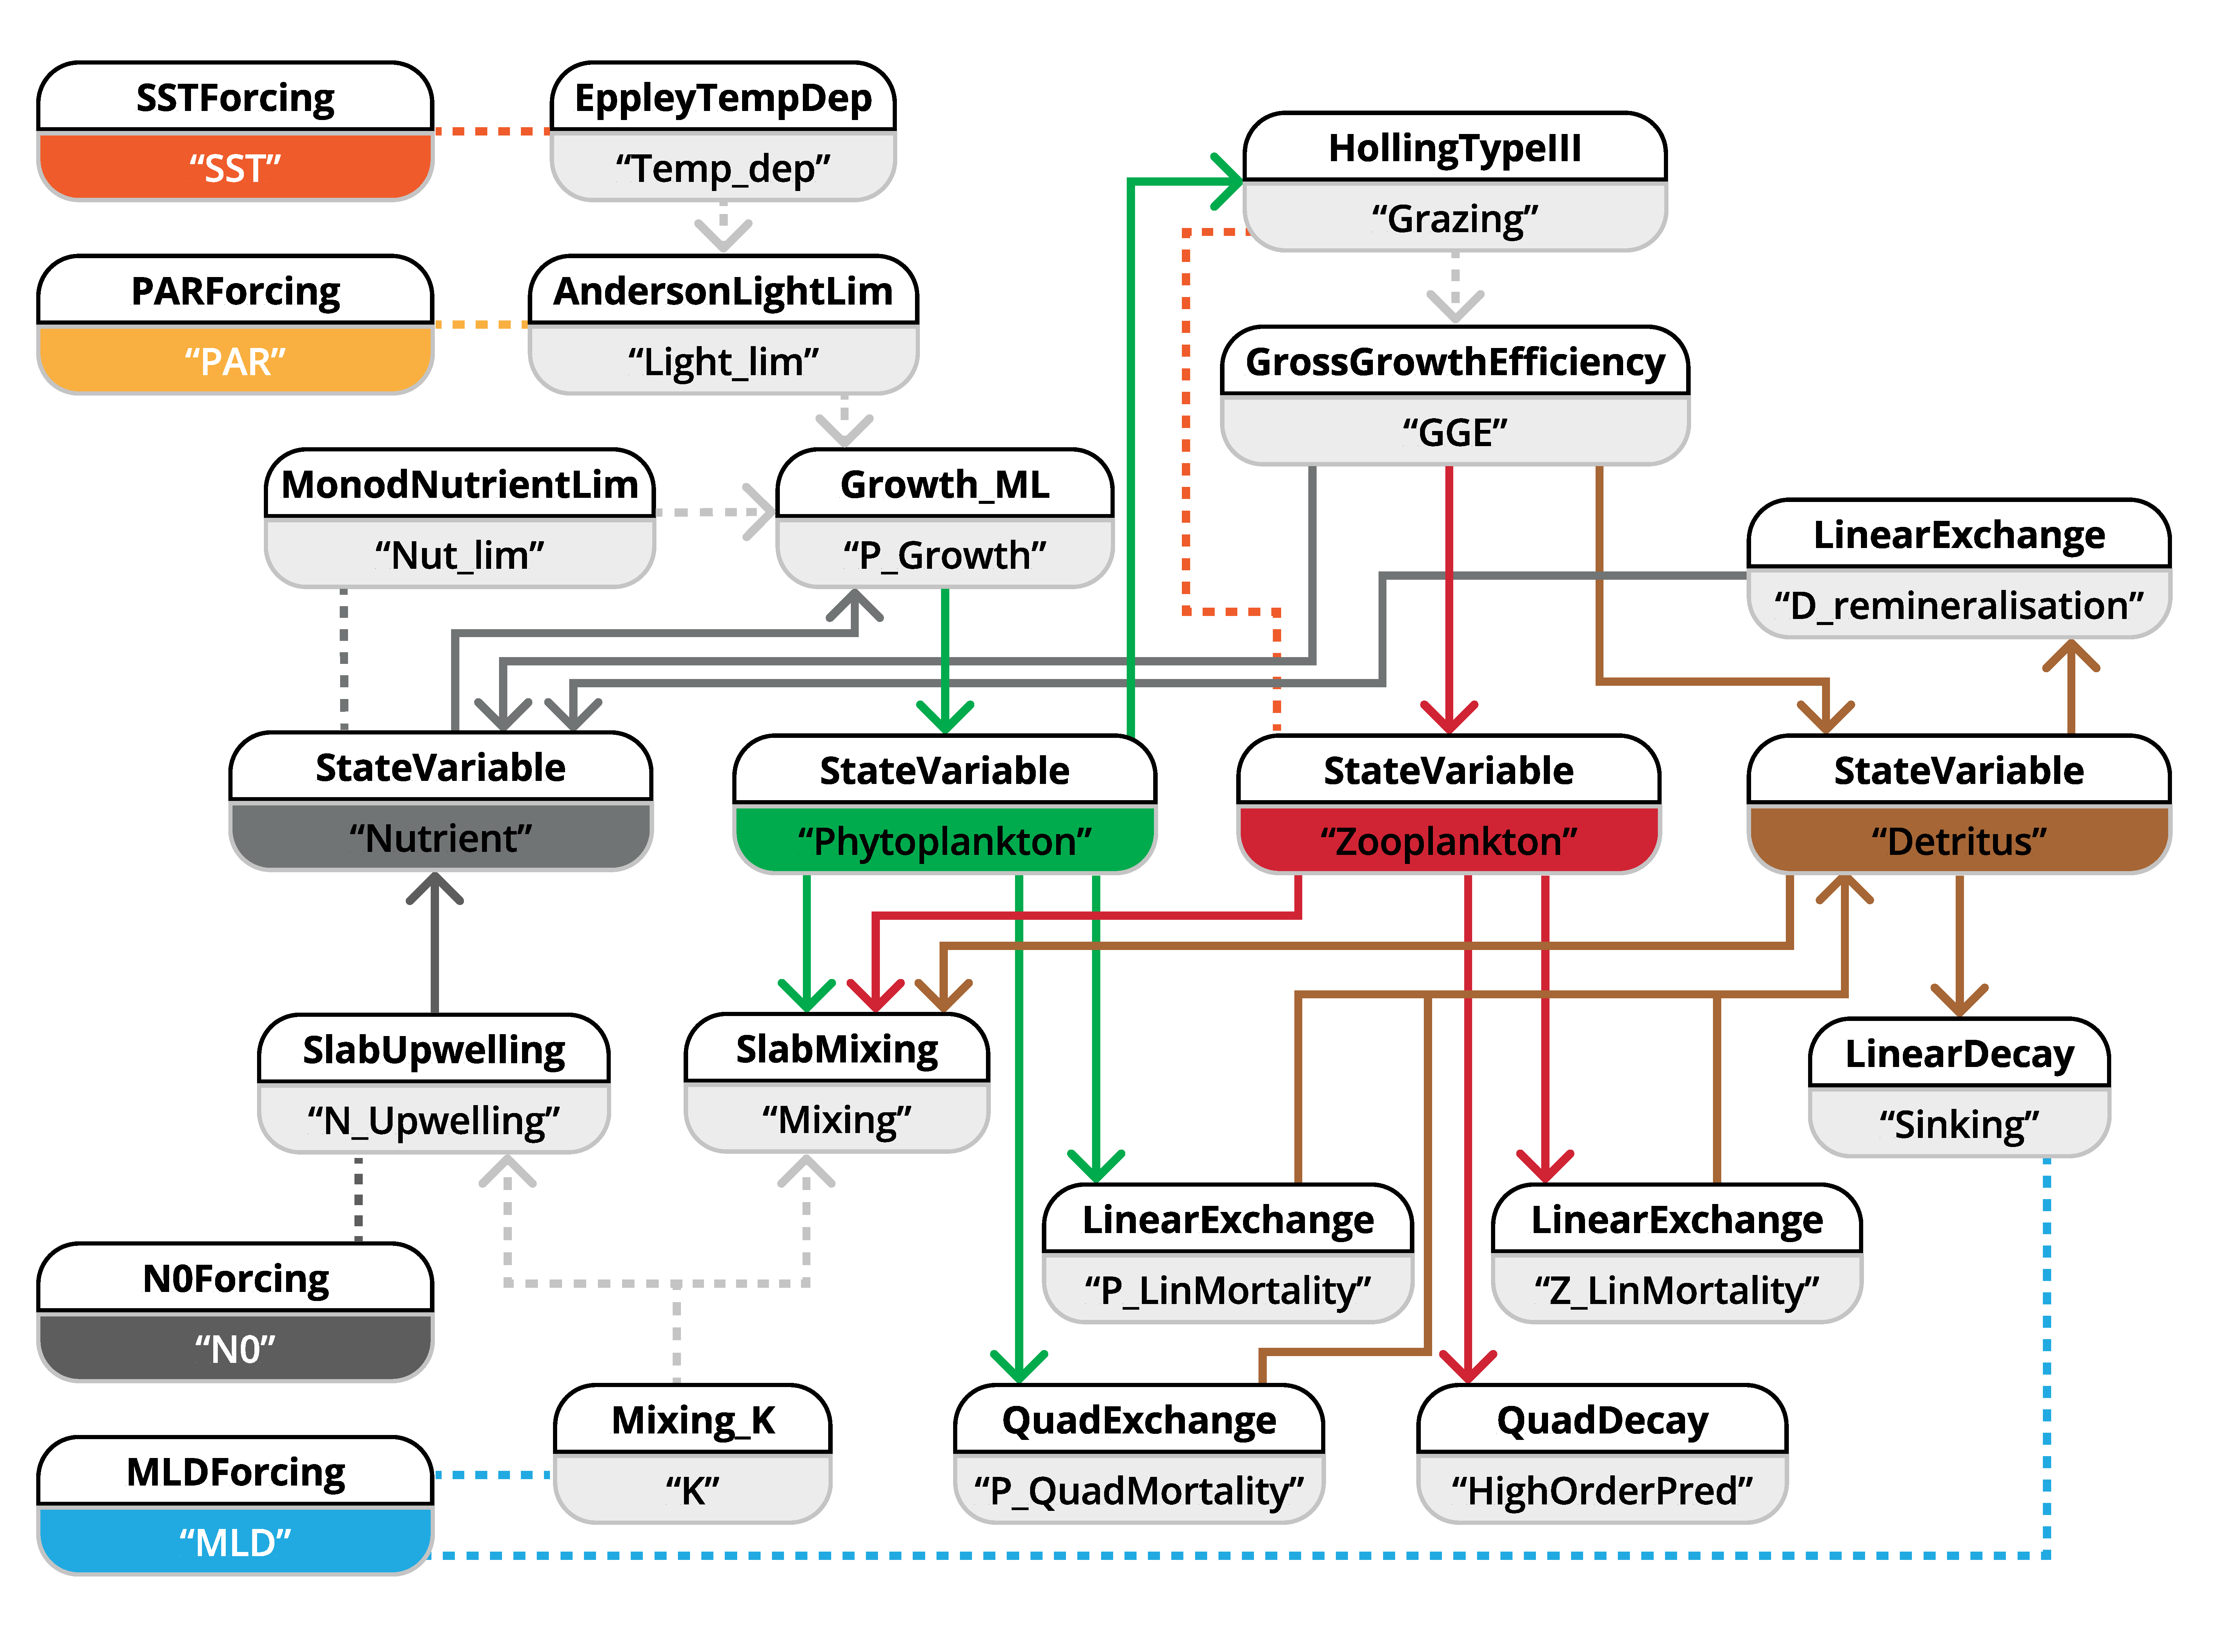
\includegraphics[width=15cm]{Figures/firstdraft_schematics/code_schematics/EMPOWER.pdf}
\caption{Schematic of use case 2 model as implemented in the XSO framework and included in the Phydra library. To simplify visualisation, only the XSO components with their labels and linkage are shown. Each component consist of a number of variables, forcings or parameters. Solid arrows indicate the flow of a flux between state variables. Dashed arrows visualise flux values passed along as group variables. Dashed lines connecting processes indicate variables and forcings passed along via their label.}
\label{Figure:CodeSchematics_2}
\end{figure*}

The NPZD slab model was implemented using the XSO framework. In order to find a useful structuring of model components, we can separate the model into state variables, forcings and fluxes. For state variables we have nutrient ($N$), phytoplankton ($P$), zooplankton ($Z$) and detritus ($D$). Forcings to the model are the mixed layer depth ($H$), nutrient concentration below the mixed layer ($N_0$), temperature in the mixed layer ($T$) and irradiance at surface ($I$). The model defines at least ten unique fluxes: Phytoplankton growth, zooplankton grazing, nutrient upwelling, mixing, sinking, remineralisation, in addition to four mortality terms.

The ecological description of our model system is adapted from the EMPOWER model, however the technical implementation using the XSO framework is quite different from the procedural R script that the model was implemented in by \citet{Anderson2015c}. Instead of using hard-coded flags to choose different ecological formulations, the XSO component structure provides open modularity and interchangeability. We appreciate the choice of transparently including the solving algorithm in the model code, however our project aims at maximum flexibility and usability. The XSO framework defines functions irrespective of the specific time-step used for evaluation and logically separates the solving algorithm from the model code into the XSO backend. This allows defining the model formulation irrespective of the complex nested for-loop structure used in the original implementation. Adding and removing state variables is also simplified, as allocating resources and storing variables in model output is handled by the framework based on the components defined at model creation.

The amount of fluxes and interdependencies between the calculations in this model require a more complex component structure than our first presented use case. In model construction, we have to find a balance between component refactoring and structural simplicity. Our goal was to allow for every individual ecologically relevant term to be exchangeable, for example each growth-limiting term was defined via an individual component. The "group variable" feature of the XSO framework allows for such a setup, so that as long as another flux defined in a component matches the group label in another component, it will be used for calculating the bulk flux defined there. The group variable can collect multiple fluxes to sum or multiply over, but it can also be used to split the calculation of a single flux between two components.

One particular example of this is that we implemented a component calculating the mixing coefficient $K$, which is computed there and passed along to calculate nutrient upwelling and the mixing fluxes of phytoplankton, zooplankton and detritus. Also there is growth limitation, which is a multiplicative process of a the growth limiting terms. Fluxes defined with a group label can in turn take a group variable as input, as was done with the temperature dependent maximum photosynthetic rate, which is passed along to calculate light limitation, which in turn is used to calculate the total growth flux. This feature was used frequently to handle the complexity of the presented model, for further detail see the description of the individual components below.

The model was implemented using 23 separate model components as visualized in Figure \ref{Figure:CodeSchematics_2}. We chose to simplify the schematic by only showing the components with their respective labels, for a detailed view of each component please consult the Phydra repository on Github.

The model processes and their respective components are listed below, with a short description of their function and application in the model:

\begin{enumerate}
    \item State variables:
    \begin{itemize}
        \item \texttt{StateVariable}: This simple component defines a state variable within the XSO framework and was used to register the state variables $N$, $P$, $Z$ and $D$. At model creation the label of the component (e.g. "Nutrient") is supplied, while the label for the variable used to link fluxes to the variables (e.g. "N") is supplied at model setup.
    \end{itemize}
    
    \item Slab-ocean forcings:
    \begin{itemize}
        \item \texttt{MLDForcing}: The mixed layer depth forcing is read from a file, interpolated and supplied via the label \texttt{"MLD"} to the framework. 
        \item \texttt{N0Forcing}: The forcing for nutrient below the mixed layer is read from a file, interpolated and supplied via the label \texttt{"N0"} to the framework. 
        \item \texttt{PARForcing}: This component contains the light submodel, calculating irradiance climatology for the station locations.
        \item \texttt{SSTForcing}: The forcing for temperature within the mixed layer is read from a file, interpolated and supplied via the label \texttt{"SST"} to the framework.
    \end{itemize}
    
    \item Slab-ocean physics:
    \begin{itemize}
        \item \texttt{Mixing\_K}: From the forcing supplied via \texttt{MLDForcing} the mixing coefficient $K$ is calculated once and supplied to \texttt{SlabUpwelling} and \texttt{SlabMixing} via a group variable. $K$ is thus calculated only once per time-step for more efficient computation.
        \item \texttt{SlabUpwelling} calculates nutrient upwelling via the value of $K$ and the difference between the $N_0$ forcing and $N$. 
        \item \texttt{SlabMixing} employs the list-input functionality described in the first use case, and calculates the effect of mixing on $P$, $Z$ and $D$. Finally, 
        \item \texttt{SlabMixing} also receives the MLD forcing ($H$) from \texttt{MLDForcing} and calculates the sinking flux acting on $D$.
    \end{itemize}
    
    \item Phytoplankton growth: Temperature-dependent, light- and nutrient-limited growth of phytoplankton is another model process that was implemented with multiple linked components, to allow for greater flexibility.
    \begin{itemize}    
        \item \texttt{GrowthML} is the process that receives all the separate terms and calculates the net growth flux from a group variable. 
        \item \texttt{TempDepGrowth} calculates the maximum photosynthetic rate and passes the result along as a group variable to \texttt{SmithLightLim}. The temperature forcing ($T$) is supplied via the \texttt{SSTForcing} component.
        \item \texttt{SmithLightLim} calculates the integrated light limitation based on the maximum photosynthetic rate passed from \texttt{TempDepGrowth}. The forcing of irradiance at surface ($I$) is passed from the \texttt{PARForcing} component.
        \item \texttt{MonodGrowthLim} calculates nutrient-limitation dependent on the ambient nutrient concentration $N$ based on Monod kinetics. 
    \end{itemize}
    
    \item Zooplankton grazing: The grazing flux is set up via two components, that are linked via a group variable.
    \begin{itemize}    
        \item \texttt{HollingType3} calculates the total grazing fluxes that subtract from $P$ and $D$. [Explain Holling Type 3 shortly]. \texttt{HollingType3} was implemented with a list input for the resource variable, so that it would be simple to add or remove state variables from the zooplankton prey pool. The grazing preference is supplied as a list of the same dimension, where the order of values has to correspond to the order of supplied labels for the resource variable. 
        \item \texttt{GrowthGrowthEfficiency} receives the array of grazing fluxes ($P$ to $Z$ and $D$ to $Z$) and handles the routing of the total grazed biomass into three fractions, that are assimilated to $Z$, egested to $D$ and excreted to $N$ respectively.
    \end{itemize}
    
    \item Detritus remineralisation:
    \begin{itemize}
        \item \texttt{LinearExchange} takes a source and sink variable as input, as well as a rate parameter ($m_D$ in this case) and transfers that fraction from $D$ to $N$.
    \end{itemize}
    
    \item Mortality fluxes: Mortality fluxes can similarly be implemented using basic components from the Phydra library.
    \begin{itemize}
        \item \texttt{LinearExchange} calculates the linear mortality terms of $P$ and $Z$, both feeding into $D$. 
        \item \texttt{QuadExchange} implements quadratic phytoplankton mortality, as it feeds into $D$. 
        \item \texttt{QuadDecay} calculates higher-order mortality of zooplankton that is lost from the system.
    \end{itemize}
\end{enumerate}

% Probably the forcing plot can go in the appendix?
%%f
\begin{figure*}[t]
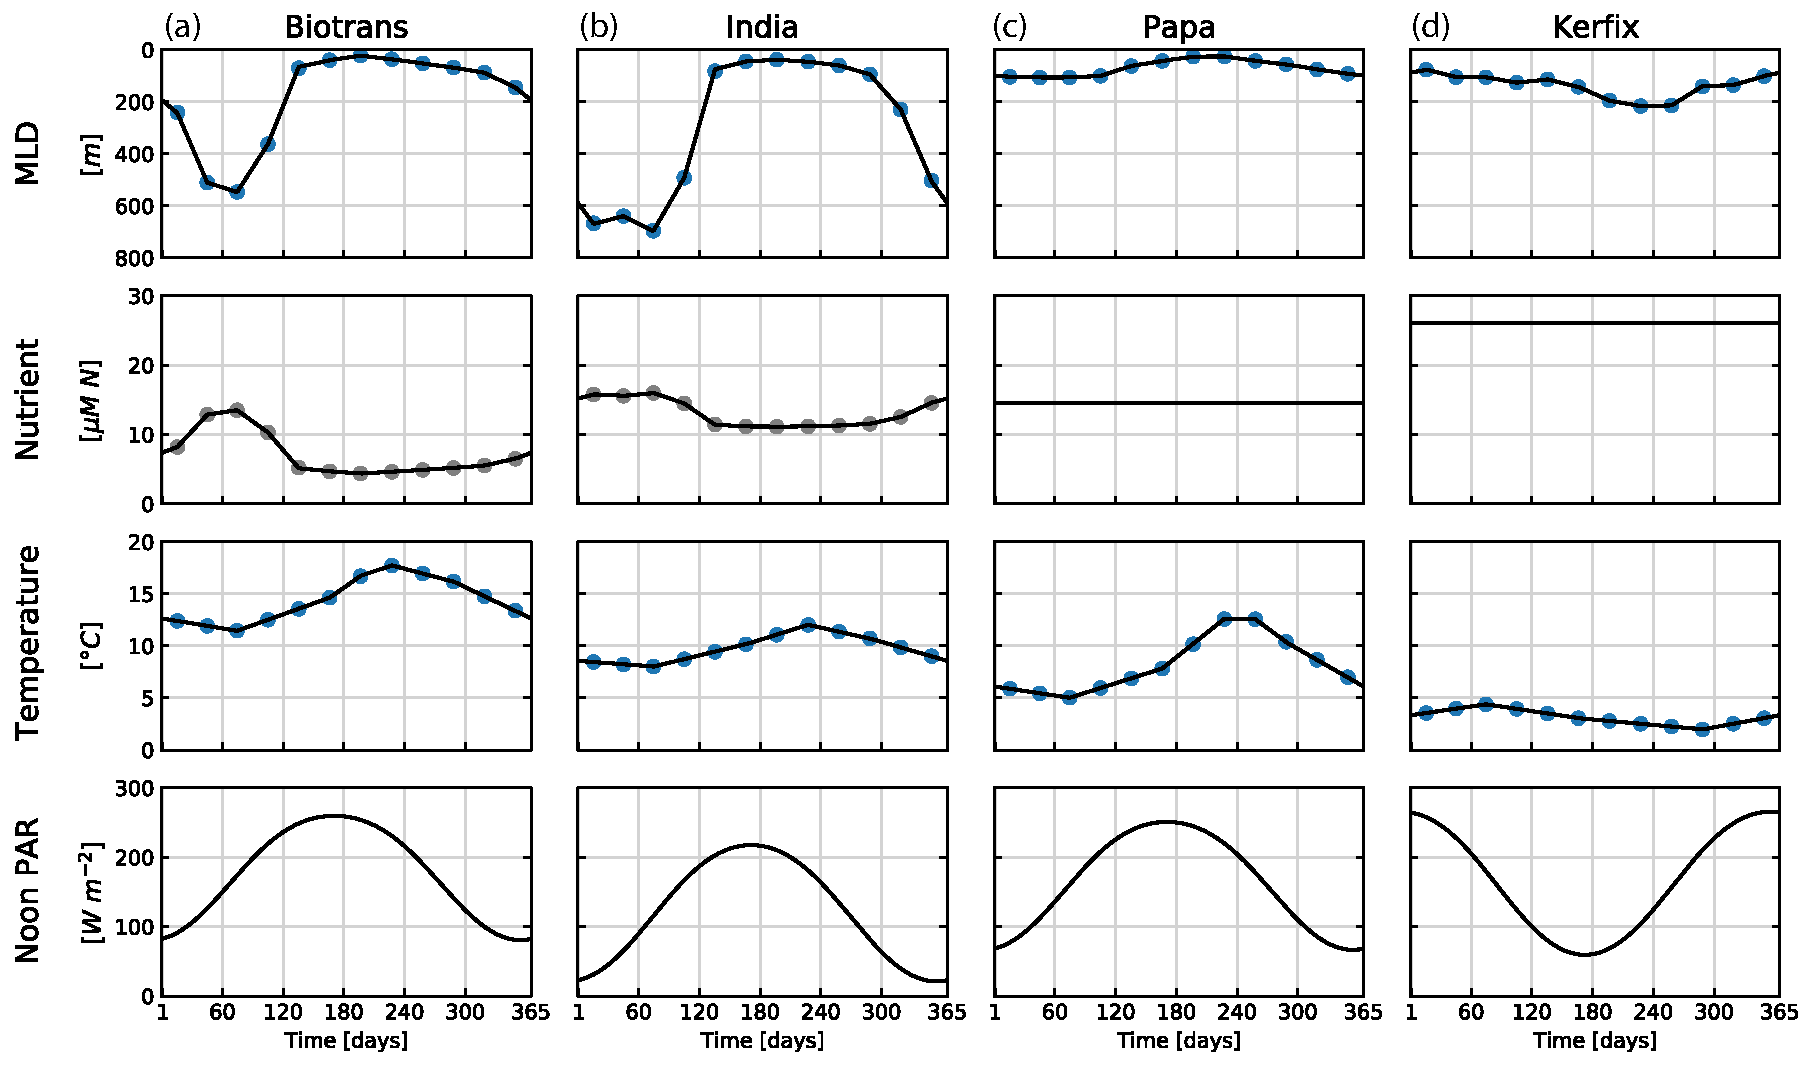
\includegraphics[width=15cm]{Figures/firstdraft_plots/02_EMPOWER_forcing.pdf}
\caption{Forcing is shown for the four locations: Mixed Layer Depth ($H$), Nitrate below the Mixed Layer ($N_0$), irradiance at surface ($I$) and temperature averaged across the mixed layer ($T$). Mixed layer depth and temperature data from Anderson et al. 2015. Nutrient forcing is a function of depth for locations Biotrans and India, and a constant value for Papa and Kerfix. Irradiance is calculated as a function of latitude.}
\label{Figure:EMPOWERforcing}
\end{figure*}

We followed \citet{Anderson2015c} in running the model in four exemplary ocean stations (BIOTRANS, India, Papa and KERFIX). The NPZD slab model is driven by four periodic external forcings shown in figure \ref{Figure:EMPOWERforcing}, that follow the approach used in the original publication but were extracted from updated data sources. 
The forcing for mixed layer depth ($H$) is taken from an updated version of the IFREMER MLD climatology  \citep{DeBoyerMontegut2004} including more data and using an optimized estimation of MLD, that was kindly supplied by Clement de Boyer Montegut.
The nutrient concentration below the mixed layer ($N_0$) is calculated from a combination of the MLD climatology and depth-resolved climatology for nitrate in the World Ocean Atlas (WOA) 2018 \citep{Garcia2019WORLDSilicate}. The temperature of the mixed layer ($T$) similarly calculated using the MLD climatology and the temperature data of WOA 2018 \citep{Locarnini2019WorldTemperature}.
The forcing for irradiance at surface ($I$) is calculated via a light submodel, that employs trigonometric/astronomical equations to calculate light climatology for a location, given the latitude and cloud fraction as input parameters. The specific model used by \citet{Anderson2015c} was adapted from \citet{Shine1984ParametrizationAlbedo}.

From satellite data we can retrieve actual measurements of photosynthetically active radiation for the locations, which removes the mathematical complexity of utilizing a light submodel. 
%perhaps we can actually use satellite PAR for our model runs?? Will be much simpler to implement.
Although not shown in this publication, Phydra includes a component that provides the satellite forcing for the four stations. The modular structure easily allows switching the \texttt{PARForcing} component from one forcing to the other.

As detailed in section \ref{Section:ComponentBuildingBlocks}, forcing from data needs to be interpolated to be compatible with an adaptive step-wise solver such as SciPy's odeint algorithm used here. In the original EMPOWER implementation a linear interpolation method is used. In testing different interpolation methods, we found that smoothing the forcing will result in much less variable model output for the shown state variables. We follow \citet{Anderson2015c} in linearly interpolating our forcing, since we wanted to recreate the original model output. All forcing is taken from climatological data which is inherently smoothed and integrated both temporally and spatially, so the rapid changes in the derivative created via linear interpolation could be considered an artifact of the interpolation method, The authors wanted to note that choosing the interpolation method can have drastic effects on model output and needs to be considered carefully.


Following \citet{Anderson2015c}, the model is compared to seasonal data for nitrate within the mixed layer and chlorophyll concentration at all four stations. We used updated versions of the original data sources to retrieve the verification data. Nitrate within the mixed layer is calculated from a combination of the WOA 2018 nitrate data and the IFREMER MLD Climatology used for the $N_0$ forcing. Chlorophyll data is from MODIS aqua chlorophyll climatology \citep{NASAGoddardSpaceFlightCenterOceanEcologyLaboratoryOceanBiologyProcessingGroup}. We did not follow the approach of taking a median year for chlorphyll data, since the forcing is also climatology data and we do not assume to be able to replicate particular biomass peaks of certain years. The climatological data follows the general pattern shown in the chlorophyll data used as verification data in the original paper.


The parameters used in model runs are adapted from \citet{Anderson2015c}, see table \ref{Table:EMPOWERparams} for a complete list of parameters for all four stations.

%%% TWO-COLUMN TABLE
%
%t
\begin{table*}[t]
\caption{Model parameters used in runs for use case 2 for the four stations:}
\begin{tabular}{l c c c c c r}
\tophline
Parameter & Description & BIOTRANS & India & Papa & KERFIX & Units \\
\middlehline

$V_P^{max}$ & max. rate of photosynthesis at 0 \unit{\degree C} & 2.5 & 2.5 & 1.25 & 1.25 & \unit{g C (g chl)^{-1} h^{-1}}\\
$\alpha$ & initial slope of P-I curve & 0.15 & 0.15 & 0.075 & 0.075 & \unit{g C (g chl)^{-1} h^{-1}}\\
$k_N$ & half-sat. const: N uptake & 0.85  & 0.85  & 0.85  & 0.85 & \unit{µM \ N} \\
$m_P$ & linear P mortality & 0.015 & 0.015 & 0.015 & 0.015  & \unit{d^{−1}} \\
$m_{P2}$ & quadratic P mortality & 0.025 & 0.025 & 0.025 & 0.025 & \unit{(µM \ N)^{-1} d^{−1}} \\
$\mu_Z$ & Z max. ingestion rate & 1.0 & 1.0 & 1.25 & 2.0 & \unit{d^{−1}} \\
$k_Z$ & Z half-saturation for intake & 0.6 & 0.6 & 0.6 & 0.6 & \unit{µM \ N} \\
$\varphi_P$ & grazing preference: P & 0.67 & 0.67 & 0.67 & 0.67 & \\
$\varphi_D$ & grazing preference: D & 0.33 & 0.33 & 0.33 & 0.33 & \\
$\beta_Z$ & Z absorption efficiency & 0.69 & 0.69 & 0.69 & 0.69 &\\
$k_{NZ}$ & Z net production efficiency & 0.75 & 0.75 & 0.75 &  0.75 &\\
$m_Z$ & linear Z mortality  & 0.02 & 0.0 & 0.02 & 0.02 & \unit{d^{−1}} \\
$m_{Z2}$ & quadratic Z mortality & 0.34 & 0.34 & 0.34 & 0.34 & \unit{(µM \ N)^{-1} d^{−1}}  \\
$v_D$ & D linear sinking rate & 6.43 & 6.43 & 6.43 & 6.43 & \unit{m \ d^{−1}}\\
$m_D$ & D remineralisation rate & 0.06 & 0.06 & 0.06 & 0.06 & \unit{d^{−1}} \\
$\kappa$ & constant mixing parameter & 0.13 & 0.13 & 0.13 & 0.13 & \unit{m \ d^{−1}}\\
$\theta_{chl}$& constant mixing parameter & 75 & 75 & 75 & 75 & \unit{g \ g^{−1}} \\

\bottomhline
\end{tabular}
\label{Table:EMPOWERparams}
\belowtable{These parameters were adapted from \citet{Anderson2015c}} % Table Footnotes
\end{table*}
%

The batch dimension feature of the XSO model setup function presented in section \ref{Section:Workflow:ModelSetup} was utilized here. It allows defining a new dimension at model setup and supplying a list of values for a specific parameter. In our case this additional dimension defines the four stations via the specific forcing and the parameters $V_P^{max}$, $\alpha$, $\mu_Z$ and $m_Z$ that \citet{Anderson2015c} varied between the locations. At runtime the model is solved individually for each set of parameters in the supplied lists and output is returned in a single Xarray dataset. The model output for each station can then be easily retrieved via the supplied batch dimension label (in this case \texttt{"station"}). In our presentation we limited ourselves to recreating the model runs shown in the original publication, but this feature also lends itself well for parameter scans and further testing of the model.

\citet{Anderson2015c} included a detailed discussion of the treatment of light in a slab model. From the formulations presented in the original paper we adapted two implementations of the analytic depth integral of light. These are a simple Beer's law, which parameterizes light attenuation with a single attenuation coefficient for the entire mixed layer, as well as the more complex piecewise description originally presented in \citet{Anderson1993APhotosynthesis}, which evaluates light attenuation for three discrete depth intervals within the mixed layer as a function of chlorophyll concentration with specific polynomial coefficients for each interval. Model results for both formulations are shown and compared below.

\subsubsection{Results}
%%f
\begin{figure*}[t]
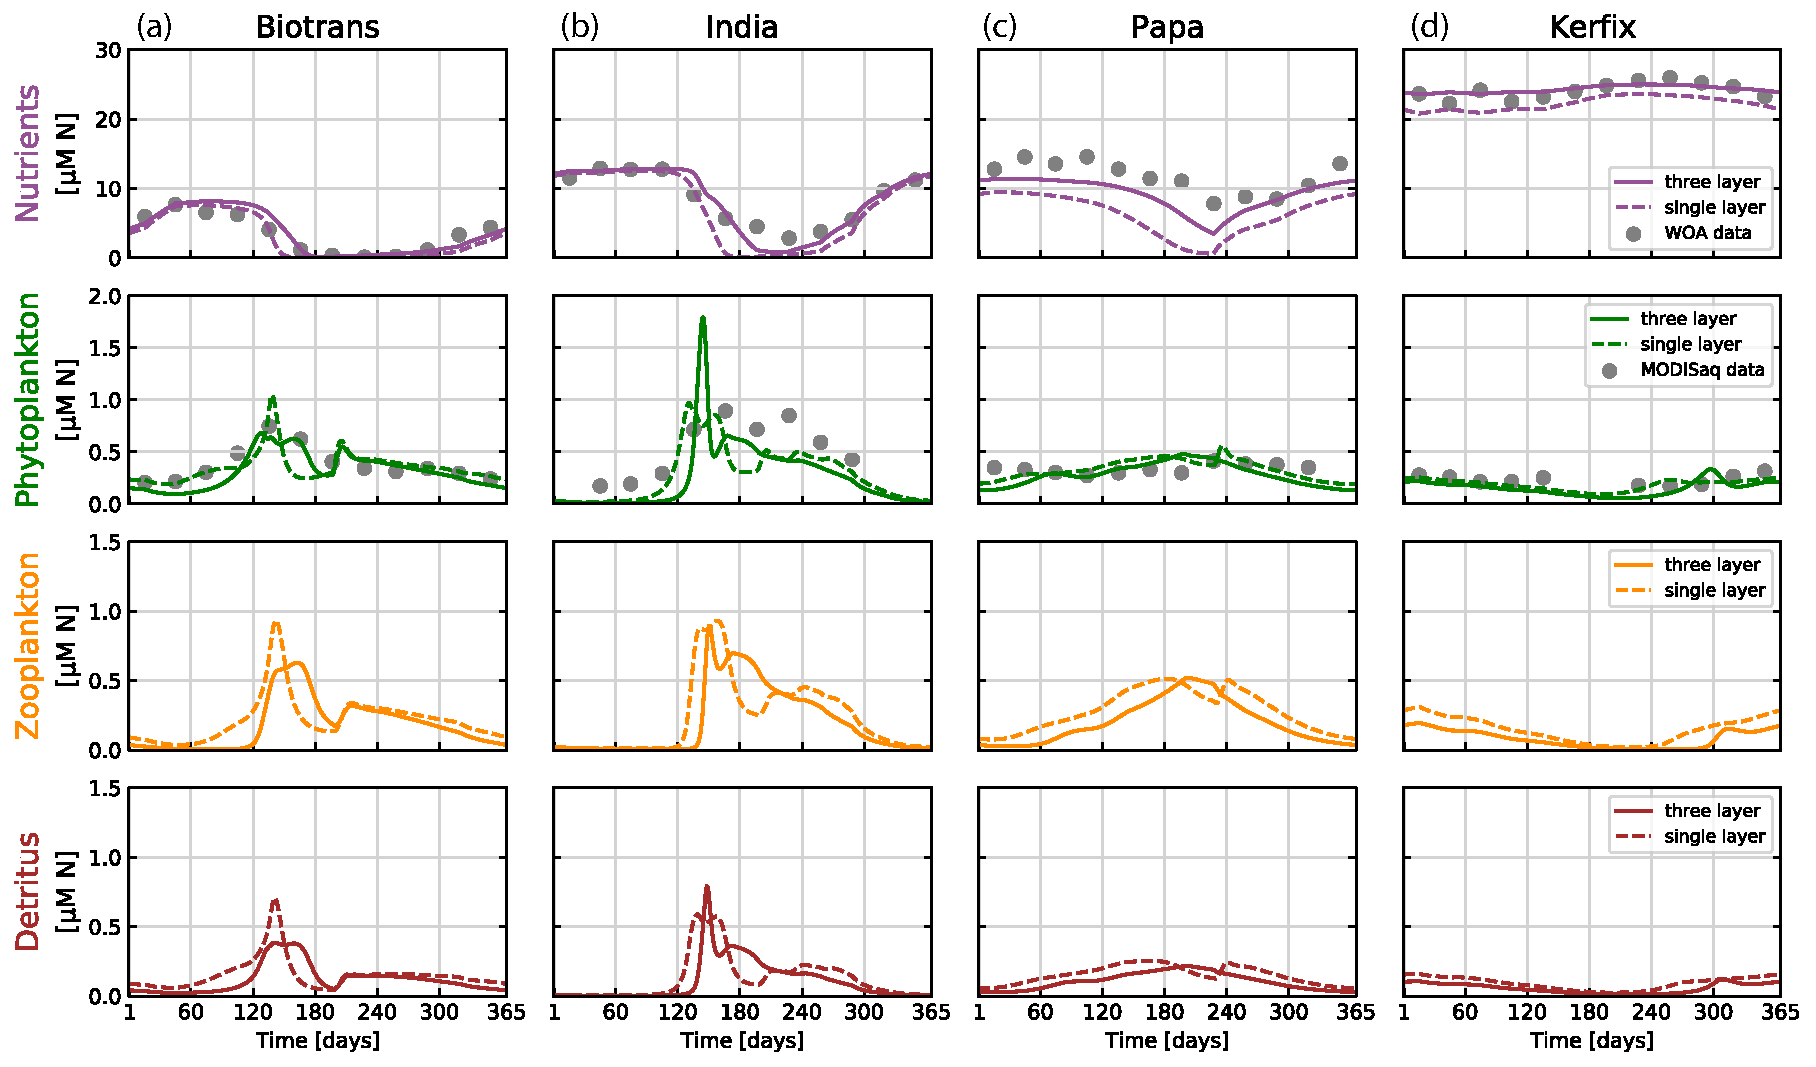
\includegraphics[width=15cm]{Figures/firstdraft_plots/02_EMPOWER_lightcomp.pdf}
\caption{Comparative slab model runs, EMPOWER model locations and forcing. Final year of a five year run. Three layer model of light attenuation in the mixed layer is thick line. Single layer model is dashed line. Verification data for Nitrogen in the upper mixed layer is taken from WOA 2018. Phytoplankton verification data is monthly climatology derived from MODIS aqua observations, C-to-Chlorophyll ratio of 75 is assumed in model and used to calculate conversion, in addition to a Redfield ratio of 16:1 for C-to-N.}
\label{Figure:ResultsEMPOWER}
\end{figure*}

Model output for all state variables and the four stations is shown in figure \ref{Figure:ResultsEMPOWER}. Output of the model for both the simple and piecewise formulation of Beer's law are shown in solid and dashed lines respectively. 
Despite the different technical implementation and solving algorithms employed here, the model output of our implementation closely matches the dynamics shown in the original paper. Since parameter tuning was performed by \citet{Anderson2015c}, the overall dynamics of nutrients and phytoplankton show a good agreement with the climatological data from the four stations. The more complicated piecewise Beer's law shows better agreement with the data, particularly for station Papa. This seems to be a result of greater light limitation of phytoplankton growth, as nutrient draw-down during growth periods is consistently lower when compared to the simple Beer's law.

We show that our framework can recreate the model and results shown by \citet{Anderson2015c}, and present the model in a flexible modular framework, that allows further experimentation and testing of different model structures.


\subsection{Model use case 3: A complex size-based NPZ model - ASTroCAT}

From a model describing an oceanic physical setting with a relatively simple ecosystem, we move to a model with a simplified physical setting with a complex description of a size-structured ecosystem. The model structure for the second use case was adapted from the ATroCAT model \citep{Banas2011b}. The original publication features extended investigation of model dynamics, for example under variable forcing or with stochastic grazing parameters. We focus on the basic setup under constant forcing. It is a simple box model that features an allometric description of multiple size-classes of both phytoplankton growing on a single nutrient, as well as an equal amount of size-classes of zooplankton grazing on phytoplankton. This level of trophic interaction is highly resolved, but many other ecological processes are neglected, e.g. there is no detrital or regeneration pathway. Even in this simple box-model setting, the complex food web yields an emergent pattern of phytoplankton size diversity. 

Size is called a "master-trait" in the trait-based description of plankton ecology, allowing modellers and ecologist to describe the diverse plankton community along one continuous axis \citep{Litchman2008}. 

Combining the dimension functionality of the XSO framework with the built-in vectorization of model equations lends itself very well to implement such a model. Instead of defining state variable without dimensionality, as was done in the previous two use cases, we simply add a dimension label and can initialize and use the variable instead as an array of size-classes. The number of size-classes is inherently variable and can be set at model setup. We showcase this feature by running the model with 2 to 50 clones and comparing bulk phytoplankton biomass between runs.

\subsubsection{Description}
%%f
\begin{figure}[t]
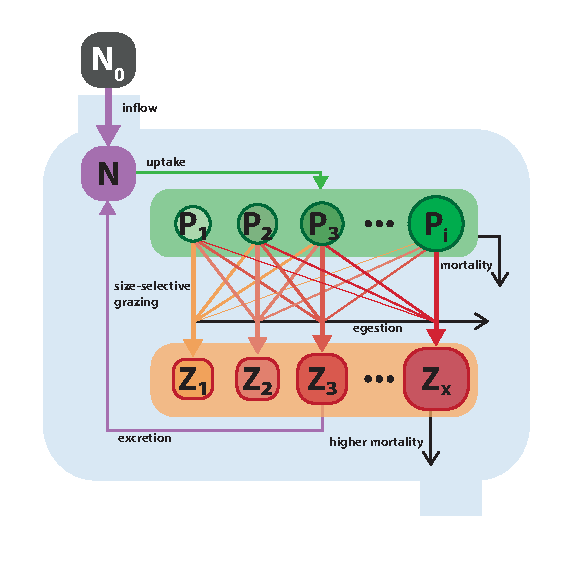
\includegraphics[width=8.3cm]{Figures/firstdraft_schematics/03_schematics_ASTroCAT.pdf}
\caption{Model schematic of size-structured $NP_{i}Z_{j}$ trophic model. Model structure and parameterisation is adapted from \citet{Banas2011b}.}
\label{Figure:ModelSchematics_3}
\end{figure}

For the second use case we have implemented a size-spectral NPZ ecosystem model as presented in Figure \ref{Figure:ModelSchematics_3}. It uses nitrogen as its currency (quantities are measured in units of $\mu mol$ N $m^{-3}$, or $\mu M$), with state variables for dissolved nutrient $N$ and multiple size classes of both phytoplankton $P_i$ and zooplankton $Z_j$. 
This model use case employs a simple box as physical setting. Inflow of nutrients is the only external input into the system, whilst mortality processes and a part of the grazing flux are removed from the system completely. Model structure and parameterisation is adapted from the ASTroCAT model \citep{Banas2011b}.

The model describes a size-structured community of phytoplankton and zooplankton, with each state variable defined by their equivalent spherical diameter (ESD). In model runs presented in this paper, we follow \citet{Banas2011b} in running simulations with 40 size classes of equally log-spaced ESD of $P$ (1 to 20 \unit{\mu m}), and 40 matching classes of $Z$ (2.1 to 460  \unit{\mu m}). Additionally we perform an experiment where the number of size classes within these ranges is varied from 2 to 50.
The model can be defined with any number of size classes within meaningful boundaries of the allometric parameterisation. Size classes are denoted by the subscript $i$ for phytoplankton and $j$ for zooplankton. In the implementation of a size-spectral model by \citeauthor{Banas2011b} the food-web is implicitly made up of matching pairs of $P_i$ and $Z_j$, to avoid creating classes within the size spectrum that are artificially released or suppressed by grazing pressure.

%\subsubsection{Nutrient}
Dissolved inorganic nitrogen (DIN) in the model system ($N$) is supplied from influx of medium with nutrient concentration $N_0$ at a constant rate $f$ and the fraction of grazed biomass that is excreted by $Z$. The concentration $N_0$ and the flow rate $f$ determine the total nutrient supply to the system. Zooplankton excretion is a recycled term, that also adds back into the pool of $N$. The only loss term of $N$ is phytoplankton growth.

%\subsubsection{Phytoplankton}
Phytoplankton biomass for each size class $P_i$ increases through nutrient-limited growth. Nutrient limitation of phytoplankton growth $\gamma_i^N$ is described by the Michaelis-Menten (or Monod) equation:

\begin{equation}
    \gamma_i^N =  \frac{N}{k_N^i + N} 
\end{equation}

where $k_N^i$ is the size-dependent half-saturation constant and $N$ is ambient nutrient concentration in the medium.

Non-grazing mortality of phytoplankton is described the factor $m^P$ that is scaled by the maximum intrinsic growth rate $\mu_{max}^i$, so that $m^P \mu_{max}^i$ yields the specific mortality rate for each size class. This accounts for natural mortality and excretion.

%\subsubsection{Zooplankton}
Zooplankton size class $Z_j$ grazing on phytoplankton size class $P_i$ is calculated by
\begin{equation}
    G_P^{ij} = \mu_j^Z \ \frac{ \varphi_{ij} \cdot P_i }{ k_Z + \sum_{i}(\varphi_{ij} \cdot P_i) } \ Z_j
\end{equation}
where $\mu_Z^j$ is the size-dependent maximum ingestion rate, $k_Z$ is the prey half-saturation level and $\varphi_{ij}$ is the relative preference of $Z_j$ for prey type $P_i$.

Prey preference is assumed to vary with phytoplankton size $size_{P}^i$ in a log-Gaussian distribution around an optimal prey size for each grazer $size_{opt}^j$.
\begin{equation}
    \varphi_{ij} = exp \left[ -\left( \ \frac{ log_{10}(size_P^i) - log_{10}(size_{opt}^j) }{ \Delta size_{P} } \right) \right]
\end{equation}
Where $\Delta size_{P}$ is the prey size tolerance parameter, with units of \unit{log_{10}(\mu m)}, that controls the width of the Gaussian distribution.

Zooplankton growth is a product of total biomass grazed ($G_P$) and the net production efficiency parameter $\epsilon$, for which values between 0.2 and 0.3 have been observed for a wide range of zooplankton  \citep{Straile1997GrossGroup}. Excretion of grazed biomass to $N$ is parameterized by $f_{eg}$ and another egested fraction that would feed into a detrital pool is lost from the system. Following \citet{Banas2011b} the grazing fractions are split equally ($\epsilon = f_{eg} = 1/3$).

Zooplankton experiences quadratic mortality according to the parameter $m_{Z2}$, describing higher-order mortality and predation of zooplankton that is removed from the system following \citet{Edwards2000TheModels}. This closure term is quadratic, calculated with the implicit assumption that mortality of $Z_j$ is proportional to total zooplankton biomass $\sum_{j} Z_j$.

%\subsubsection{Model equations}
The rates of change of the state variables are described by the following set of equations. See \citet{Banas2011b} for a more detailed discussion of model structure and formulation.

\begin{equation}
    \frac{d N}{d t} = 
    f \ N_0 % Nutrient mixing
    +  f_{eg} \ \sum_{j} \sum_{i} G_P^{ij} % Unassimilated grazing by Z
    - \sum_{i} ( \mu_{max}^i \ \gamma_i^N \ P_i) % Phytoplankton gains
\end{equation}

%PHYTOPLANKTON
\begin{equation}
    \frac{d P_i}{d t} =
    \mu_{max}^i \  \gamma_i^N \   P_i  % Phytoplankton gains
    - m_P  \ \mu_{max}^i \ P_i % Linear mortality
    - \sum_{j} G_P^{ij} % Z grazing
\end{equation}

%ZOOPLANKTON
\begin{equation}
    \frac{d Z_j}{d t} =
    \epsilon \ \sum_{i} G_P^{ij} % Assimilated grazing
    - m_{Z2} \ Z_j \ \sum_{j} Z_j  % Quadratic mortality
\end{equation}

\subsubsection{Implementation}
%%f
\begin{figure*}[t]
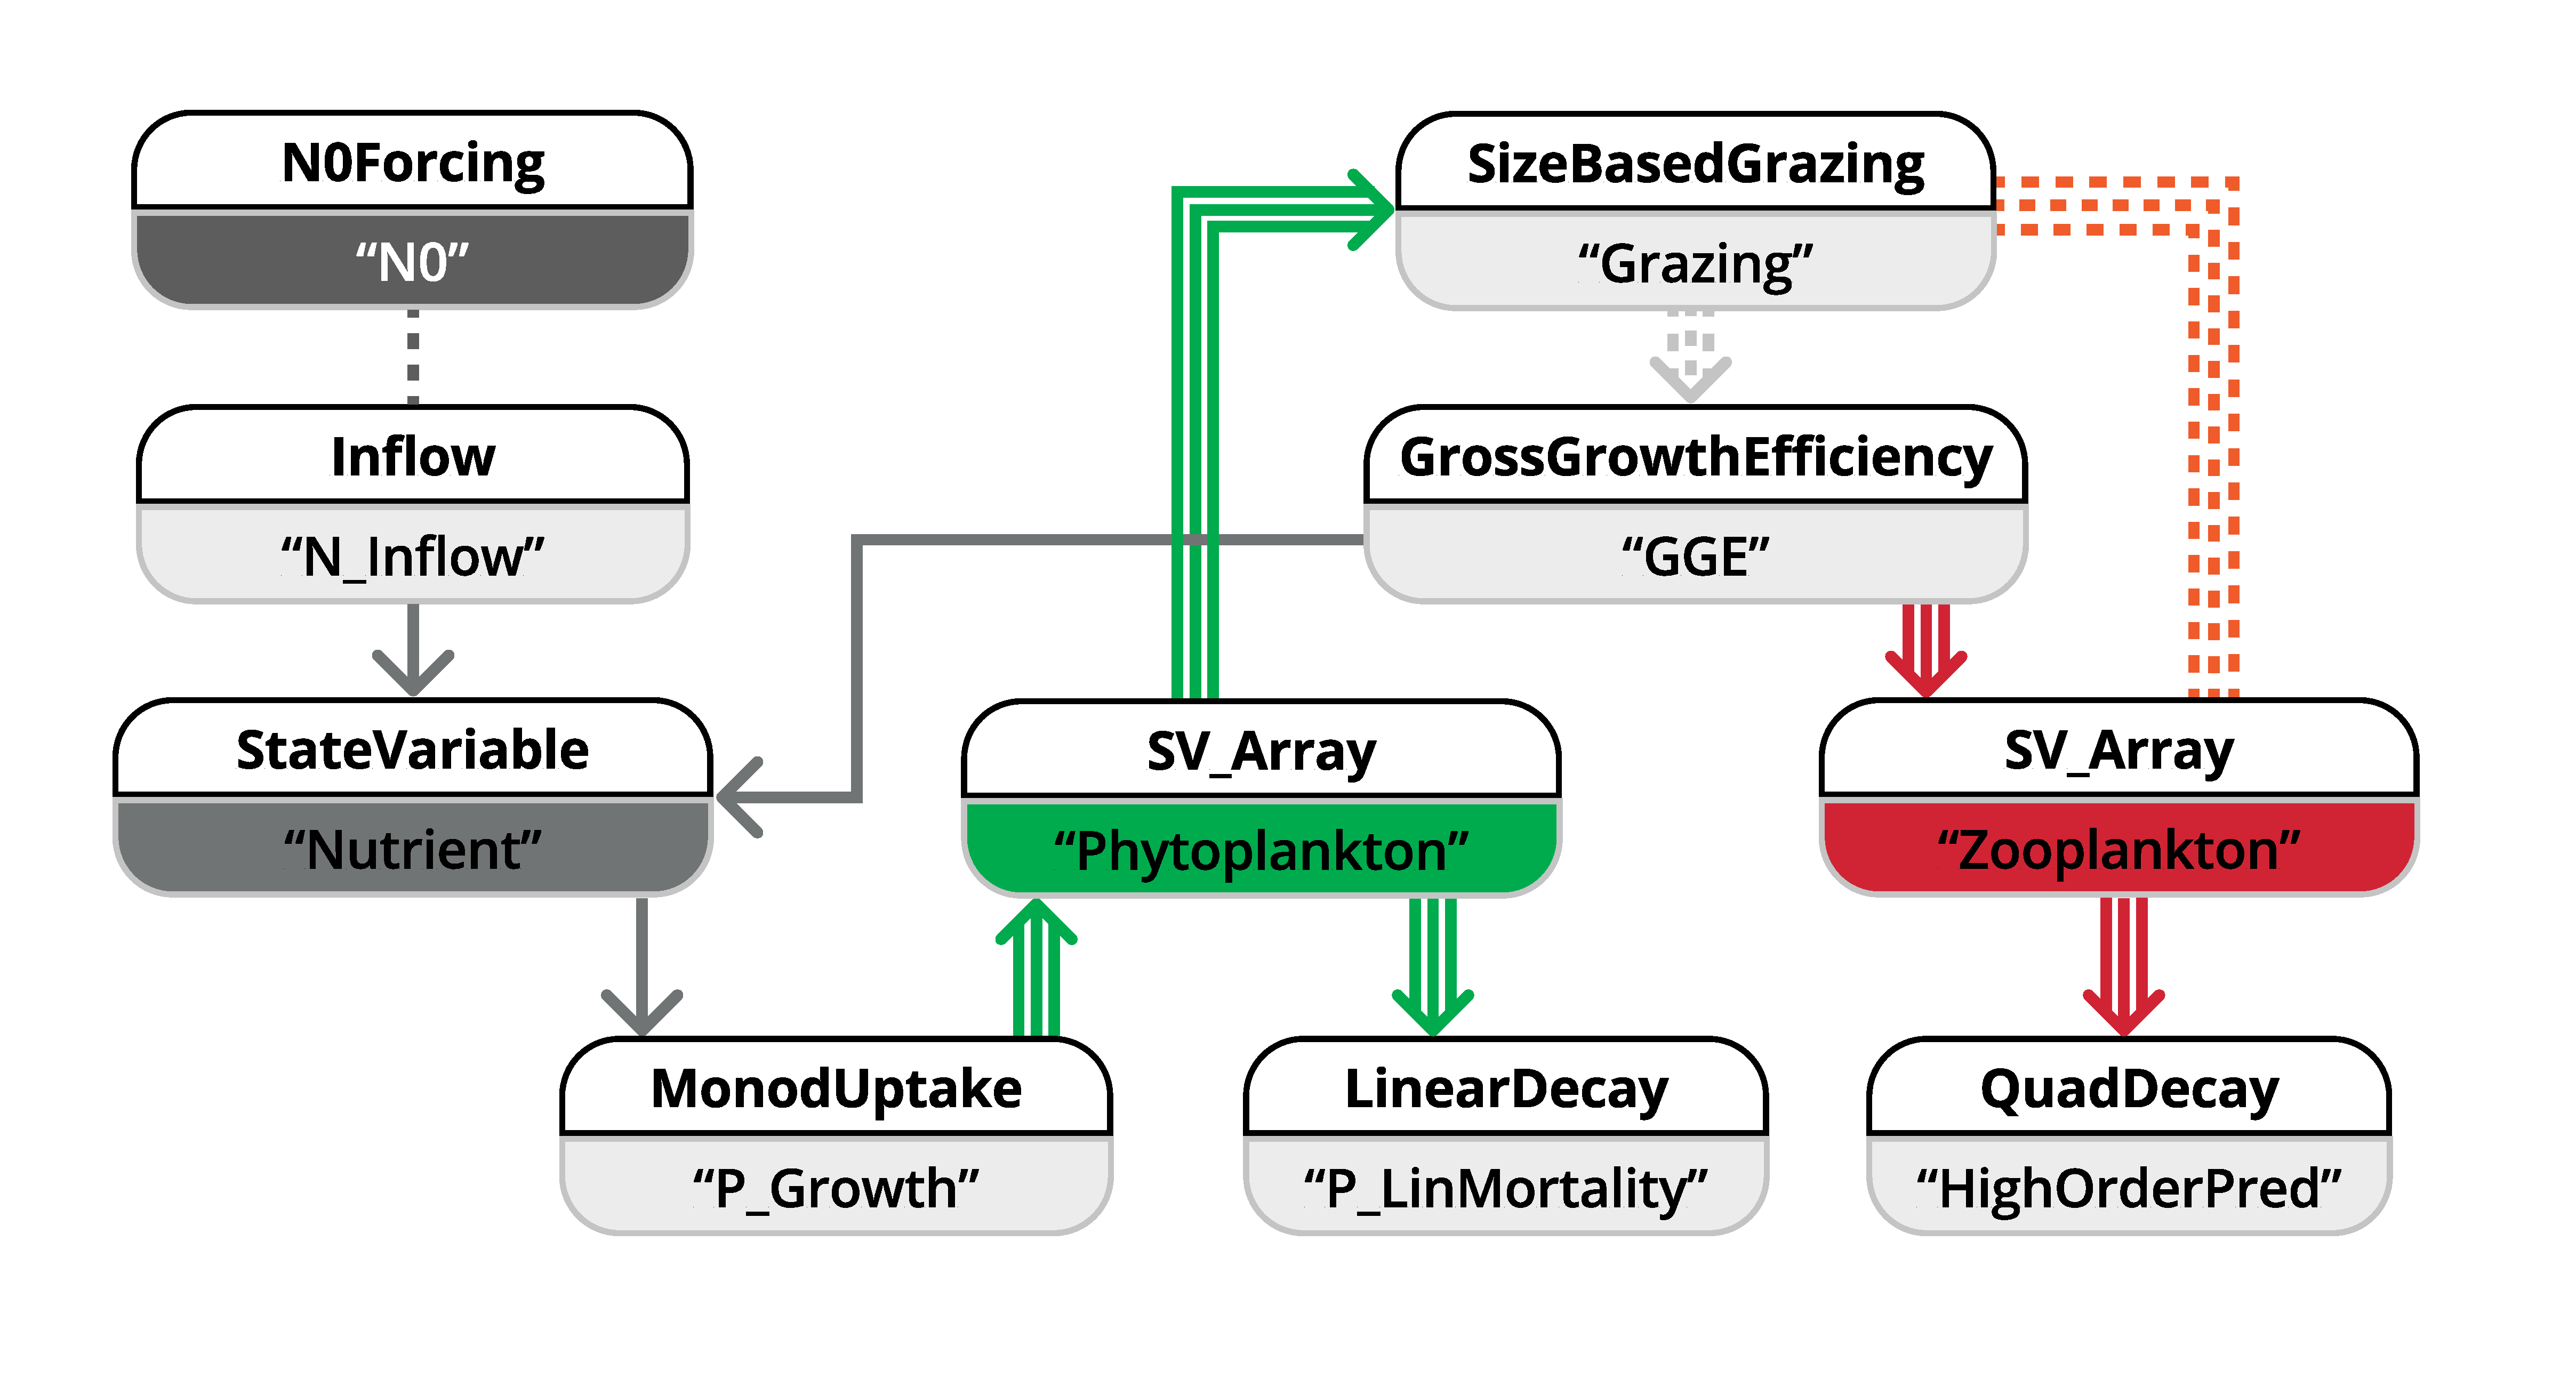
\includegraphics[width=15cm]{Figures/firstdraft_schematics/code_schematics/ASTroCAT.pdf}
\caption{Schematic of use case 3 model as implemented in the XSO framework and included in the Phydra library. To simplify visualisation, only the XSO components with their labels and linkage are shown. Each component consist of a number of variables, forcings or parameters. Solid arrows indicate the flow of a flux between state variables. Dashed arrows visualise flux values passed along as group variables. Dashed lines connecting processes indicate variables and forcings passed along via their label. Arrows with multiple lines indicate values with dimensions that are passed along.}
\label{Figure:CodeSchematics_3}
\end{figure*}

The ASTroCAT model was implemented using the XSO framework. In order to find a useful structuring of model components, we can separate the model into state variables, forcings and fluxes. For state variables we have the nutrient ($N$), multiple size-classes of phytoplankton ($P_i$) and zooplankton ($Z_j$). The only forcing is the nutrient concentration of the external medium ($N_0$). At least 5 fluxes can be separately defined: The inflow of the external medium, $P_i$ growing on $N$, $Z_j$ grazing on $P_i$ and mortality terms for both $P_i$ and $Z_j$.
The model was implemented using 10 XSO components as visualized in Figure \ref{Figure:CodeSchematics_3}. We chose to simplify the schematic by only showing the components with their respective labels. A detailed description of each component can be found in the Phydra repository on Github.

The original ASTroCAT model was implemented with an interactive graphical user interface showing beautiful animation of model output that was written in Processing 2 and kindly supplied by the author upon request. Our implementation in the XSO framework is technically quite similar to the original model code, with the major differences being the modular component structure and the use of vectorization instead of for-loops to define functions computing the \textit{fluxes} acting on arrays of size-classes.

The model processes and their respective components are listed below, with a short description of their function and application in the model:

\begin{enumerate}
    \item State variables: 
    \begin{itemize}
        \item \texttt{StateVariable}: This is the same component used in the previous use cases. It registers the state variable for the ambient nutrient concentration ($N$). 
        \item \texttt{SVArraySize}: This is an extension of the \texttt{StateVariable} component, that additionally defines a dimension for the state variable and stores the array of sizes via a parameter. The supplied dimension label allows initializing a state variable as an array within the XSO framework, that is also represented in the Xarray data structure of the model setup and output. The number of values in the state variable array can be supplied flexibly at model setup by passing a list or array of that dimension as initial values. Across the model the framework will check that labelled dimensions share the same number of values. The label of the state variable (\texttt{"P"} and \texttt{"Z"} in this case) remains a single string and can be used across the model to reference the entire array. In this model we can use the same component (with the same dimension label) to register $P_i$ and $Z_j$, as the model was constructed for both of these to share the same number of dimensions.
    \end{itemize}

    \item Nutrient influx: 
    \begin{itemize}
        \item \texttt{ConstantForcing}: This component registers the external nutrient forcing ($N_0$) and is the same component that was applied in the first use case model.
        \item \texttt{Inflow}: The inflow flux is defined here, again this is the same implementation as in the first use case model. It adds to $N$ the flux defined as $N_0$ multiplied by a \texttt{rate} parameter. 
    \end{itemize}
    
    \item Nutrient uptake and phytoplankton growth: 
    \begin{itemize}
        \item \texttt{MonodUptake}: Similar to the nutrient influx components, this is a copy of the same component used in the first use case model, with the modification that we supply a dimension label to the \texttt{consumer} state variable and the parameters for \texttt{halfsat} and \texttt{mu}. We supply the label \texttt{"P"} for the \texttt{consumer} state variable. To set up the allometric parameters for the maximum growth rate and half-saturation constant, we calculate the parameters outside of the model definition and supply the values as a list at model setup.
    \end{itemize}
    
    \item Zooplankton grazing on phytoplankton: 
    \begin{itemize}
        \item \texttt{SizeBasedGrazing}: The grazing formulation for the multiple size classes of phytoplankton and zooplankton is the most complex function presented in our use cases. Care needs to be taken with proper handling of the dimensions within the function, but if it is done correctly the built-in vectorization of the XSO framework allows efficient calculation of the matrix-wise interaction for any number of size-classes. To improve the modularity of our implementation we split the calculation of the grazing matrix from the routing of the fluxes to their sources and sinks. This can be achieved via the group functionality of XSO, passing along the full matrix as a group variable to the \texttt{SizeBasedGrazing\_Fluxes} component. At model setup, the \texttt{SizeBasedGrazing} takes the label for resource and consumer, as well as the feeding preference matrix, the array of maximum ingestion rates and the single $k_Z$ parameter as input.
        \item \texttt{SizeBasedGrazing\_Fluxes}: This component receives the full matrix of grazing fluxes ($P_i$ over $Z_j$) as a group variable from the \texttt{SizeBasedGrazing} component and allocates the summed up fluxes to the sources and sinks of the grazing flux. Summing over $Z_j$ yields the array of grazing fluxes subtracting from $P_i$, while summing over $P_i$ and multiplying by the assimilation coefficient $\epsilon$ yields the array of grazing fluxes assimilated to $Z_j$. Summing over the entire matrix and multiplying by $f_{eg}$ yields the excreted biomass adding to $N$. At model setup, the component takes the respective labels of the state variables, as well as the parameters for $\epsilon$ and $f_{eg}$ as input.
    \end{itemize}
    
        \item Zooplankton and phytoplankton mortality: 
    \begin{itemize}
        \item \texttt{LinearDecayDim}: Linear mortality of phytoplankton can be defined with the same component employed in the first use case, with the modification that a dimension label is supplied as an argument to the flux and state variable. 
        \item \texttt{QuadDecayDim}: Similarly quadratic mortality of zooplankton is defined with a dimension label. The vectorization functionality allows defining the quadratic term as the sum of all zooplankton biomass, while still calculating over all zooplankton size classes.
    \end{itemize}
\end{enumerate}

The distribution of phytoplankton and zooplankton sizes are log-spaced. The \texttt{SVArraySize} \textit{component} registering the phytoplankton and zooplankton state variables takes the size range as parameter input, however this is only for documentation purposes. The allometric parameters are calculated via helper functions outside of model \textit{components} to allow maximum flexibility and reduce complexity of the specific model implementation.

Parameters were adapted from \citet{Banas2011b}, see table \ref{Table:usecase3parameters} for all used parameter values and allometric relationships.
\begin{table*}[t]
\caption{Parameters and allometric functions used in use case 3.}
\begin{tabular}{l c c r}
Parameter & Description & Value & Units \\
\tophline
$f$ & Flow rate of external nutrient & 1 & \unit{d^{-1}} \\
$N_0$ & External nutrient concentration & 1 & \unit{µM \ N} \\
$k_Z$ & Prey half-saturation constant & 3 & \unit{µM \ N}\\
$\Delta size_{P}$ & Prey size tolerance & 0.25 &  \\
$m_P$ & Mortality fraction of $\mu_{max}^i$ for $P_i$ & 0.1 & \unit{d^{-1}}\\
$\epsilon$ & Zooplankton growth efficiency & 0.33 & \\
$f_{eg}$ & Fraction of grazing egested & 0.33 & \\
\\

$\mu_{max}^i$ & Maximum growth rate of $P_i$ & $ 2.6 \left( \frac{size_i^{P}}{1\mu m} \right)^{-0.45}$  & \unit{d^{-1}} \\
$k_N^i$ & Nutrient half-saturation constant of $P_i$ & $ 0.1 \left( \frac{size_i^{P}}{1\mu m} \right)$ & \unit{µM \ N} \\

$\mu_Z^j$ & Maximum ingestion rate of $Z_j$ & $26 \left( \frac{size^i_{P}}{1\mu m} \right)^{-0.4}$ &\unit{µM \ N} \\

$size_{opt}^j$ &  & $0.65 \left( \frac{size_{P}^i}{1\mu m} \right)^{0.56}$ & \ \unit{µM \ N} \\

\bottomhline
\end{tabular}
\belowtable{Sources for allometric functions: \citep{Tang1995TheRespiration, Eppley1969HalfSaturationPhytoplankton, Hansen1997ZooplanktonRange, Hansen1994a}} % Table Footnotes
\label{Table:usecase3parameters}
\end{table*}
%

\citet{Banas2011b} present a detailed analysis of model output for variable metrics of ecosystem complexity. We recreate a part of the analysis with a simple comparison of model dynamics for a variable number of phytoplankton and zooplankton size classes. The number of state variables can be varied at model setup by supplying a list of initial values with the desired dimensions. We run the model for the range of 2 to 50 size classes.

\subsubsection{Results}
%%f
\begin{figure}[t]
\includegraphics[width=8.3cm]{Figures/firstdraft_plots/03_ASTroCAT_N50P50Z.pdf}
\caption{Nutrient concentration and biomass under steady nutrient forcing in model run resolving 50 size classes. Size classes are log-spaced in a range of 1 to 20 \unit{µ m} for phytoplankton and 2.16 to 420 \unit{µ m} for zooplankton. (a) Nutrient concentration over time. (b) Phytoplankton biomass by size class over 10 years of model time evolution. (c) Zooplankton biomass over the same period.}
\label{Figure:ResultsASTroCAT_1}
\end{figure}

Running the model with 40 size classes of phytoplankton and zooplankton recreates the dynamics presented by \citet{Banas2011b}. See figure \ref{Figure:ResultsASTroCAT_1} for the time evolution of $N$, $P_i$ and $Z_j$ over a ten year run. The complex food web shows oscillatory changes in biomass between the state variables with periods from days to years, that reach a stable distribution after 5-6 years of run time. Despite the feedback loops built into the food web, the model reaches a stable steady-state in longer runs (not shown here) and does not show chaotic behaviour.

%%f
\begin{figure}[t]
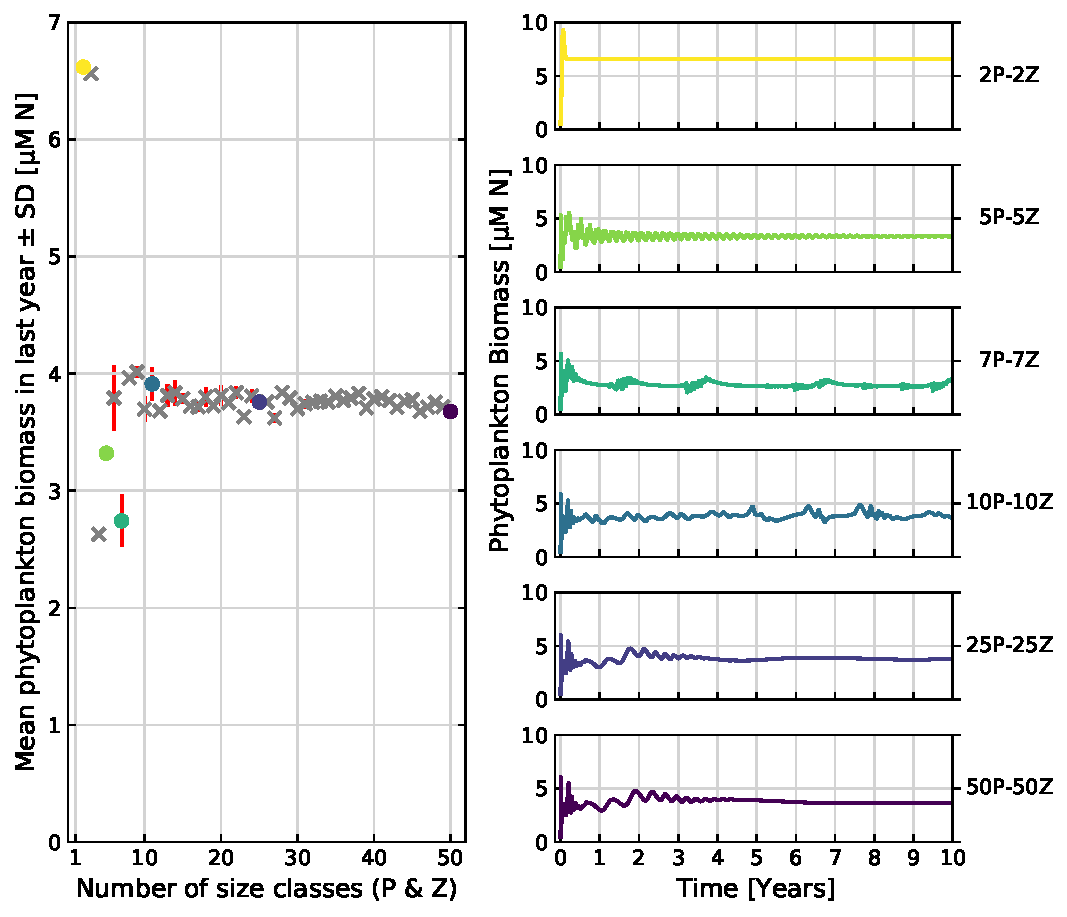
\includegraphics[width=8.3cm]{Figures/firstdraft_plots/03_ASTroCAT_sizeclassrange.pdf}
\caption{Comparative runs of varying number of size-classes. (a) Mean biomass of phytoplankton over the last year of a ten year run over a range of 2 to 50 size-classes of phytoplankton and zooplankton. Standard deviation is plotted in red. Grey crosses mark runs not otherwise shown, colored dots correspond to exemplary runs. (b) Exemplary model runs. Sum of phytoplankton biomass is shown over a ten year run.}
\label{Figure:ResultsASTroCAT_2}
\end{figure}

In figure \ref{Figure:ResultsASTroCAT_2} we show the effect on bulk phytoplankton biomass when running the model with a variable number of size classes. Lower number of size classes (2-10) show highly variable output during and for the final year of a ten year run. Bulk dynamics seems to stabilize for numbers of size classes above 10, however there is still deviation between runs in average phytoplankton biomass for the last year of model runs for more than 10 size classes. The increased resolution seems to reduce the perturbations carried on from initial model conditions, confirming the patterns observed by \citet{Baird2010IncreasingErrors}.


\section{Discussion}

\subsection{Structuring complex marine ecosystem models in a flexible framework}
- Mention the model use cases, and how complexity was handled there

An ecosystem model tracks chemical compounds as well as organisms via state variables. These state variables can define completely different components of a model, or represent a functional group. Components within Phydra are defined at this higher level and can contain a single state variable or an array of state variables that share common fluxes with differing parameterisation. Each state variable is added to the model with a specific label that is used to reference this component in all processes affecting or dependent on it.

The actual dimensions of a functional group are initialized after passing a parameter at model setup. This has been designed for easily testing different levels of ecosystem complexity.

In addition to size, the component could be modified to include information on units or other specific parameters relevant to the model. The added flexible dimensionality of components was designed with the current issues in marine ecosystem model in mind. The effects of different levels of complexity, in the number and definition of phytoplankton functional types (PFT) for example, is not routinely tested in marine ecosystem models. Phydra provides a framework that allows for easy testing through flexible modification of such model complexity at model setup.

The first release of Phydra provides only scalar and one-dimensional array implementations of state variables, but extending this to 2- and 3-dimensional flexibility is a high development priority. 
!or!
Dimensionality in state variables can be used to model functional groups or classes, as well as systems of higher dimensionality. At its current version Phydra provides only zero-dimensional models, but models of higher-dimension would be a clear next step in further development.

- XSO allows the user to choose component refactoring of model components, no limit to variable types used within a component, no limit to levels of group variables linking components to define a single ecosystem process. Fluxes could be as complex or simple as the user desires.

- Situated in complexity between GUI tools that allow drag and drop, and custom model scripts. The combination of phydra as a library and XSO as a framework aims to reduce the boilerplate code necessary to write computational models in Python.
- It would be possible to design a graphical interface for this later on, but that is not the target audience.

\subsection{Current limitations of Phydra and XSO}
- only ODE models
- presented use cases limited to zero dimensional physical settings
- limited set of solvers
- so far not optimized for very large models, reaching computational limits of implemented solvers
- less optimized than custom script (as would be expected from framework)
- no advanced features like parameter optimization yet, although technically possible
- 

\subsection{Current usage and future developments}
- The Phydra package is available via the Python pip package manager, but we encourage using Conda as a package manager that is provided with the scientific Anaconda Python distribution.
Please follow the up-to-date instructions on the Github repository for installation of Phydra and its dependencies.

% future feature development
- XSO stores model equations including the names of parameters and it would be possible to add some functions that print the mathematical equations.. which would be quite helpful to build and debug a model. (possible feature)

% CONDA NAME DROP
Since Python and the dependencies of Phydra are constantly developed further, we will provide instructions to install a fully compatible virtual environment with the Conda package manager separate from a users standard Python installation. For interactive coding and prototyping of models using Phydra, we recommend using the Jupyter environment that is available via Conda. For more complex and larger model runs on servers Python scripts are preferable.


""The framework allows to build models very quickly and dynamically from many components by automating aspects such as workflow dependencies and model input detection. It has also potential to automate other aspects like parallel execution of model components, command-line interface and/or graphical interface. It aims to ultimately help researchers forget technical aspects and stay focused on scientific developments.""

Both of Xarray-simlab and GEKKO are relatively young  Python packages and actively under development, which provides some challenges, but also allows for constant improvements to the functionality that Phydra provides.

% OPEN SOURCE CONTRIBUTION 
Phydra and XSO are open-source projects. Contributions are welcome and in fact greatly appreciated. Users can contribute in many ways by reporting bugs, submitting feedback, contributing to the development of the code or the documentation. Please read the contributing guidelines on the Github repository for further details.


%%% added Section for editing purposes, later simply use \conclusions
\section{Conclusions}
%\conclusions  %% \conclusions[modified heading if necessary]
% Place this project in the wider open science ecosystem, outlook on further developments

make the main points again (from intro)


What is Phydra? What is XSO?


Reiterate what we have written and the use cases shown


old school modeling can be done better
show that I am moving in a direction that other people are! Brian Rose climlab, etc.

- This is a first step in the direction

- package architecture is heavily borrowing from other open-source python efforts (e.g. xarray-simlab, xarray, numpy, scipy,...) 
- functionality can be merged with other open-source python projects (veros-bgcm, BGC-val)

- xsimlab is a powerful framework that is actively developed further, more added compatibilities possible
- same goes for xarray-simlab-ode, e.g. solvers, visualization, optimization of model construction \& execution in backend - much potential to develop it further
- Python lends itself well to interface with legacy fortran code, can make marine 3d modeling much more accessible without loosing performance or accuracy

- want to make the first step, hoping that people will adopt and contribute

- any modeler willing to use phydra will probably have to write his own processes, and this is also the intention. Object oriented structure still highly simplifies collaboration with non-modelers or people not versed in higher-level python. Higher transparency and collaboration between modelers as well, since same code base and similar 

e.g. next steps: 1. add 1D, 2D, 3D models 2. add agent-based models using xarray-simlab framework



%% END OF SECTION CONCLUSIONS









%% The following commands are for the statements about the availability of data sets and/or software code corresponding to the manuscript.
%% It is strongly recommended to make use of these sections in case data sets and/or software code have been part of your research the article is based on.

\codeavailability{TEXT} %% use this section when having only software code available


\dataavailability{TEXT} %% use this section when having only data sets available


\codedataavailability{TEXT} %% use this section when having data sets and software code available


\sampleavailability{TEXT} %% use this section when having geoscientific samples available


\videosupplement{TEXT} %% use this section when having video supplements available


\appendix
\section{}    %% Appendix A

\subsection{}     %% Appendix A1, A2, etc.


\noappendix       %% use this to mark the end of the appendix section. Otherwise the figures might be numbered incorrectly (e.g. 10 instead of 1).

%% Regarding figures and tables in appendices, the following two options are possible depending on your general handling of figures and tables in the manuscript environment:

%% Option 1: If you sorted all figures and tables into the sections of the text, please also sort the appendix figures and appendix tables into the respective appendix sections.
%% They will be correctly named automatically.

%% Option 2: If you put all figures after the reference list, please insert appendix tables and figures after the normal tables and figures.
%% To rename them correctly to A1, A2, etc., please add the following commands in front of them:

\appendixfigures  %% needs to be added in front of appendix figures

\appendixtables   %% needs to be added in front of appendix tables

%% Please add \clearpage between each table and/or figure. Further guidelines on figures and tables can be found below.



\authorcontribution{TEXT} %% this section is mandatory

\competinginterests{TEXT} %% this section is mandatory even if you declare that no competing interests are present

\disclaimer{TEXT} %% optional section

\begin{acknowledgements}
TEXT
\end{acknowledgements}




%% REFERENCES

%% The reference list is compiled as follows:

%\begin{thebibliography}{}

%\bibitem[AUTHOR(YEAR)]{LABEL1}
%REFERENCE 1

%\bibitem[AUTHOR(YEAR)]{LABEL2}
%REFERENCE 2

%\end{thebibliography}

%% Since the Copernicus LaTeX package includes the BibTeX style file copernicus.bst,
%% authors experienced with BibTeX only have to include the following two lines:
%%
\bibliographystyle{copernicus}
\bibliography{references.bib}
%%
%% URLs and DOIs can be entered in your BibTeX file as:
%%
%% URL = {http://www.xyz.org/~jones/idx_g.htm}
%% DOI = {10.5194/xyz}


%% LITERATURE CITATIONS
%%
%% command                        & example result
%% \citet{jones90}|               & Jones et al. (1990)
%% \citep{jones90}|               & (Jones et al., 1990)
%% \citep{jones90,jones93}|       & (Jones et al., 1990, 1993)
%% \citep[p.~32]{jones90}|        & (Jones et al., 1990, p.~32)
%% \citep[e.g.,][]{jones90}|      & (e.g., Jones et al., 1990)
%% \citep[e.g.,][p.~32]{jones90}| & (e.g., Jones et al., 1990, p.~32)
%% \citeauthor{jones90}|          & Jones et al.
%% \citeyear{jones90}|            & 1990



%% FIGURES

%% When figures and tables are placed at the end of the MS (article in one-column style), please add \clearpage
%% between bibliography and first table and/or figure as well as between each table and/or figure.

% The figure files should be labelled correctly with Arabic numerals (e.g. fig01.jpg, fig02.png).


%% ONE-COLUMN FIGURES

%%f
%\begin{figure}[t]
%\includegraphics[width=8.3cm]{FILE NAME}
%\caption{TEXT}
%\end{figure}
%
%%% TWO-COLUMN FIGURES
%
%%f
%\begin{figure*}[t]
%\includegraphics[width=12cm]{FILE NAME}
%\caption{TEXT}
%\end{figure*}
%
%
%%% TABLES
%%%
%%% The different columns must be seperated with a & command and should
%%% end with \\ to identify the column brake.
%
%%% ONE-COLUMN TABLE
%
%%t
%\begin{table}[t]
%\caption{TEXT}
%\begin{tabular}{column = lcr}
%\tophline
%
%\middlehline
%
%\bottomhline
%\end{tabular}
%\belowtable{} % Table Footnotes
%\end{table}
%
%%% TWO-COLUMN TABLE
%
%%t
%\begin{table*}[t]
%\caption{TEXT}
%\begin{tabular}{column = lcr}
%\tophline
%
%\middlehline
%
%\bottomhline
%\end{tabular}
%\belowtable{} % Table Footnotes
%\end{table*}
%
%%% LANDSCAPE TABLE
%
%%t
%\begin{sidewaystable*}[t]
%\caption{TEXT}
%\begin{tabular}{column = lcr}
%\tophline
%
%\middlehline
%
%\bottomhline
%\end{tabular}
%\belowtable{} % Table Footnotes
%\end{sidewaystable*}
%
%
%%% MATHEMATICAL EXPRESSIONS
%
%%% All papers typeset by Copernicus Publications follow the math typesetting regulations
%%% given by the IUPAC Green Book (IUPAC: Quantities, Units and Symbols in Physical Chemistry,
%%% 2nd Edn., Blackwell Science, available at: http://old.iupac.org/publications/books/gbook/green_book_2ed.pdf, 1993).
%%%
%%% Physical quantities/variables are typeset in italic font (t for time, T for Temperature)
%%% Indices which are not defined are typeset in italic font (x, y, z, a, b, c)
%%% Items/objects which are defined are typeset in roman font (Car A, Car B)
%%% Descriptions/specifications which are defined by itself are typeset in roman font (abs, rel, ref, tot, net, ice)
%%% Abbreviations from 2 letters are typeset in roman font (RH, LAI)
%%% Vectors are identified in bold italic font using \vec{x}
%%% Matrices are identified in bold roman font
%%% Multiplication signs are typeset using the LaTeX commands \times (for vector products, grids, and exponential notations) or \cdot
%%% The character * should not be applied as mutliplication sign
%
%
%%% EQUATIONS
%
%%% Single-row equation
%
%\begin{equation}
%
%\end{equation}
%
%%% Multiline equation
%
%\begin{align}
%& 3 + 5 = 8\\
%& 3 + 5 = 8\\
%& 3 + 5 = 8
%\end{align}
%
%
%%% MATRICES
%
%\begin{matrix}
%x & y & z\\
%x & y & z\\
%x & y & z\\
%\end{matrix}
%
%
%%% ALGORITHM
%
%\begin{algorithm}
%\caption{...}
%\label{a1}
%\begin{algorithmic}
%...
%\end{algorithmic}
%\end{algorithm}
%
%
%%% CHEMICAL FORMULAS AND REACTIONS
%
%%% For formulas embedded in the text, please use \chem{}
%
%%% The reaction environment creates labels including the letter R, i.e. (R1), (R2), etc.
%
%\begin{reaction}
%%% \rightarrow should be used for normal (one-way) chemical reactions
%%% \rightleftharpoons should be used for equilibria
%%% \leftrightarrow should be used for resonance structures
%\end{reaction}
%
%
%%% PHYSICAL UNITS
%%%
%%% Please use \unit{} and apply the exponential notation


\end{document}
